\documentclass[a4paper,11pt,twoside]{report}

\overfullrule=5pt % draw overfull hboxes for visual inspection

\usepackage[
	%showframe, % show frame for page margins etc.
	scale=0.75, % fraction of page width/height to use
	headheight=30pt,
]{geometry}

%\usepackage[utf8]{inputenc} % ignored with lualatex / xelatex (which are utf8-based)
\usepackage{amsmath}
\usepackage[text]{esdiff} % text-mode derivatives in textstyle
\usepackage{tensor}
\usepackage[parfill]{parskip} % new paragraph: new line, no indent
\usepackage[title]{appendix}
\usepackage[hidelinks]{hyperref} % hide colored boxes around links
\usepackage[noabbrev]{cleveref}
\usepackage[labelfont=bf]{caption} % figure title in bold

\usepackage{unicode-math} % make code display utf8 characters properly
\usepackage[cachedir=.cache_minted/]{minted}
%\setmonofont{DejaVu Sans Mono} % will affect whole document, including URLs etc.
\newfontfamily\codefont{DejaVu Sans Mono}[NFSSFamily=CodeFamily] % set mono font for minted code only
\setminted{breaklines}
\setminted{frame=single}
\setminted{breakanywhere}
\setminted{fontfamily=CodeFamily}

\usepackage{fancyhdr}
\pagestyle{fancy}
\fancyhf{}
\fancyhead[LE,RO]{\textbf{\thepage}}
\fancyhead[RE]{\leftmark}
\fancyhead[LO]{\rightmark}
\fancyfoot[CE,CO]{}

\usepackage{tikz}
\usetikzlibrary{external}
\tikzexternalize[prefix=.cache_tikz/]

\usepackage{pgfplots}
\pgfplotsset{compat=1.17}
\usepgfplotslibrary{groupplots}

%\fancypagestyle{plain}{\pagestyle{fancy}} % make chapter front pages, bibliography etc. use same style as other pages (see https://tex.stackexchange.com/a/10046)

% make consistent style also on chapter first pages, bibliography etc.
\fancypagestyle{plain}{
	\fancyhf{}
	\fancyhead[LE,RO]{\textbf{\thepage}}
}

\usepackage[style=alphabetic]{biblatex}
\addbibresource{project.bib}

\newcommand\dif{\mathop{}\!\mathrm{d}}
\newcommand{\abs}[1]{\lvert #1 \rvert}
\newcommand{\integral}[4]{\int_{#3}^{#4} #1 \dif #2}
\newcommand{\variation}[1]{\delta #1}
\newcommand{\trace}[1]{\text{tr} #1}
\newcommand{\lagr}{\mathcal{L}}
\newcommand{\diag}[1]{\text{diag} \left( #1 \right)}
\newcommand{\diffv}[2]{\frac{\variation{#1}}{\variation{#2}}}

% useful intro to Latex thesis: https://www.overleaf.com/learn/latex/How_to_Write_a_Thesis_in_LaTeX_(Part_1):_Basic_Structure

\title{Project thesis}
\author{Herman Sletmoen}
\date{\today}

\begin{document}

\maketitle
\tableofcontents
\chapter*{Notation and conventions} % do not number
\addcontentsline{toc}{chapter}{Notation and conventions} % but still display in TOC (see https://tex.stackexchange.com/a/222961)
%\markboth{NOTATION AND CONVENTIONS}{} % but still display correct header (see https://tex.stackexchange.com/a/78090)

\section*{Metric signature}

We use the $(-,+,+,+)$ metric signature.

\section*{Summation convention}

We use the Einstein summation convention, in which an index that appears once as a superscript and again as a subscript in the same term is to be summed over.
If the index is roman, the sum runs from $1$ to $3$, and if it is greek, it also runs over $0$.
For example,
\begin{equation*}
	T\indices{^\mu_\mu} = \sum_{\mu=0}^3 T\indices{^\mu_\mu}
	\quad \text{and} \quad
	T\indices{^i_i} = \sum_{i=1}^3 T\indices{^i_i}
	.
\end{equation*}

\section*{Fourier transformation}

We use the Fourier transformation convention
\begin{equation}
	f(k) = \int \dif x \, e^{i k x} f(x)
	\qquad \text{and} \qquad
	f(x) = \int \frac{\dif k}{2 \pi} \, e^{-i k x} f(k) .
\end{equation}
With this convention, the delta function $\delta(x' - x)$ is given by the highlighted part of
\begin{equation}
	f(x) = \int \frac{\dif k}{2 \pi} \, e^{-i k x} f(k)
	     = \int \dif x' \underbrace{\int \frac{\dif k}{2 \pi} \, e^{i k (x'-x)}}_{\displaystyle \delta(x'-x)} f(k) .
\label{eq:pre:delta_function}
\end{equation}

(TODO: table over all constants and notation, so I don't have to write everything in the text)

\chapter{Tolman-Oppenheimer-Volkoff equation}

TODO: write intro after I know everything we should do in this section

\section{Derivation from the Einstein field equations}
\label{sec:tov}

To analyze astrophysical objects like stars, it is of considerable interest to relate the pressure $p(x)$ and energy density $\epsilon(x)$ or mass density $\rho(x)$ at every position $x$ inside the object.
We will derive the relativistic relation between these quantities from the \textbf{Einstein field equations} \cite[equation 4.44]{ref:carroll}
\begin{equation}
	G\indices{_\mu_\nu} = R_{\mu \nu} - \frac{1}{2} R g_{\mu \nu} = \frac{8 \pi G}{c^4} T_{\mu \nu} .
	\label{eq:einstein}
\end{equation}
It describes how the geometry of spacetime, described by the Ricci tensor $R\indices{_\mu_\nu}$ and Ricci scalar $R$ that are ultimately built from the metric $g\indices{_\mu_\nu}$ and encapsulated in the Einstein tensor $G\indices{_\mu_\nu}$ (see \cref{chap:gr_summary} for a summary), responds to the presence of energy-momentum in the energy-momentum tensor $T\indices{_\mu_\nu}$.
Here, $G$ is the gravitational constant and $c$ is the speed of light.
As we later compare our findings to those of Newtonian gravity, it will be useful to connect the energy density to the mass density by the \textbf{mass-energy equivalence relation}
\begin{equation}
	\epsilon(x) = \rho(x) c^2 .
	\label{eq:tov:mass_energy_equivalence}
\end{equation}

Unless rotating very fast, stars are well approximated by spheres.
For our purposes, we therefore use the coordinates
\begin{equation}
	x^\mu = (c t, r, \theta, \phi)
	\quad \text{with} \quad
	-\infty < t < \infty, \quad
	0 \leq r < \infty, \quad
	0 \leq \theta \leq \pi, \quad
	0 \leq \phi < 2 \pi .
\end{equation}
and consider the most general line element that exhibits spherical symmetry, \cite[§ 94-95]{ref:tolman}
(TODO: do more general with $\gamma(r)$, as done in Carroll?)
\begin{equation}
	% coordinates x = (ct, r, θ, ϕ)
	\dif s^2 = -e^{2 \alpha(r)} c^2 \dif t^2 + e^{2 \beta(r)} \dif r^2 + r^2 \left( \dif \theta^2 + \sin^2 \theta \dif \phi^2 \right) .
\end{equation}

We model the interior of the star as a perfect fluid with energy-momentum \cite[equation 1.114]{ref:carroll}
\begin{equation}
	T\indices{_\mu_\nu} = \frac{1}{c^2} (\epsilon+p) U_\mu U_\nu + p g\indices{_\mu_\nu}.
\end{equation}
For a static star whose fluid is at rest, $U_\mu = (U_0, \textbf{0})$ and the normalization condition $U_\mu U^\mu = -c^2$ requires $U_0 = \pm e^\alpha c$.
We choose the positive sign so the four-velocity lies in the future light cone, as we are interested in the evolution of the star.
Then the energy-momentum tensor takes the diagonal form
\begin{equation}
T\indices{_\mu_\nu} =
\begin{bmatrix}
	\epsilon e^{2\alpha} & 0            & 0     & 0                   \\
	0                    & p e^{2\beta} & 0     & 0                   \\
	0                    & 0            & p r^2 & 0                   \\
	0                    & 0            & 0     & p r^2 \sin^2 \theta \\
\end{bmatrix}
\qquad \text{or} \qquad
T\indices{_\mu^\nu} =
\begin{bmatrix}
	-\epsilon & 0 & 0 & 0 \\
	0         & p & 0 & 0 \\
	0         & 0 & p & 0 \\
	0         & 0 & 0 & p \\
\end{bmatrix}
.
\label{eq:einstein_to_tov:T}
\end{equation}

Starting with the metric, it is now straightforward, although tedious, to compute the left side of \cref{eq:einstein} from \cref{eq:def_christoffel,eq:def_riemann_tensor,eq:def_ricci_tensor,eq:def_ricci_scalar}.
For the details, refer to \cite[equation 5.11-5.15]{ref:carroll}.
After inserting the energy-momentum tensor on the right and simplifying, we get the three independent equations
(the fourth turns out proportional to the third)
\begin{subequations}
\begin{align}
	\frac{1}{r^2} e^{-2 \beta} \left( 2 r \beta' - 1 + e^{2 \beta} \right)                               &= \frac{8 \pi G}{c^4} \epsilon
	&& \left( G\indices{_0_0} = \frac{8 \pi G}{c^4} T\indices{_0_0} \right) , \label{eq:einstein_to_tov:tt} \\
	\frac{1}{r^2} e^{-2 \beta} \left( 2 r \alpha' + 1 - e^{2 \beta} \right)                              &= \frac{8 \pi G}{c^4} p
	&& \left( G\indices{_1_1} = \frac{8 \pi G}{c^4} T\indices{_1_1} \right) , \label{eq:einstein_to_tov:rr} \\
	e^{-2 \beta} \left( \alpha'' + (\alpha')^2 - \alpha' \beta' + \frac{1}{r} (\alpha' - \beta') \right) &= \frac{8 \pi G}{c^4} p
	&& \left( G\indices{_2_2} = \frac{8 \pi G}{c^4} T\indices{_2_2} \right) . \label{eq:einstein_to_tov:thetatheta}
\end{align}
\end{subequations}

Next, let us introduce the mass of the star.
Define the function $m(r)$ by
\begin{equation}
	e^{2 \beta} = \left( 1 - \frac{2 G m(r)}{r c^2} \right)^{-1} ,
	\label{eq:einstein_to_tov:def_m}
\end{equation}
so $g\indices{_1_1}$ resembles the Schwarzschild metric element.
Then \cref{eq:einstein_to_tov:tt} becomes
\begin{equation}
	\diff{(m c^2)}{r} = 4 \pi r^2 \epsilon(r) ,
	\label{eq:einstein_to_tov:m_rho}
\end{equation}
directly relating $m(r)$ and $\epsilon(r)$.
If we set $m(0) = 0$, we can integrate to get
\begin{equation}
	m(r) c^2 = \integral{\epsilon(r') 4 \pi r'^2}{r'}{0}{r} .
	\label{eq:einstein_to_tov:m_integral}
\end{equation}
\cite[page 602]{ref:mtw} shows that setting $m(0) \neq 0$ creates a singularity at the origin, which is not physically acceptable.
Outside a star that extends to $r = R$, there is vacuum with $\epsilon = 0$ and our metric should match the Schwarzschild metric with $g\indices{_1_1} = (1-2GM/rc^2)^{-1}$ and Schwarzschild mass $M$.
By comparison with \cref{eq:einstein_to_tov:def_m}, the \textbf{Schwarzschild mass} of the star must be
\begin{equation}
	M = m(R) = \frac{1}{c^2} \integral{\epsilon(r) 4 \pi r^2}{r}{0}{R} = \integral{\rho(r) 4 \pi r^2}{r}{0}{R}.
	\label{eq:einstein_to_tov:schwarzschild_mass}
\end{equation}
It is tempting to interpret the Schwarzschild mass $M$ as the Newtonian mass of the star and \eqref{eq:einstein_to_tov:m_integral} as the volume integral of the energy density $\epsilon(r)$.
But $4 \pi r^2$ is not a proper volume element, as it does not involve the full spatial metric determinant.
We return to this question in \cref{sec:weak_field_limit} after studying incompressible stars in \cref{sec:incompressible_star}, where we will see that the first interpretation is correct, while the latter is more subtle and differs by the binding energy of the star.

Meanwhile, definition \eqref{eq:einstein_to_tov:def_m} turns \cref{eq:einstein_to_tov:rr} into
\begin{equation}
	\diff{\alpha}{r} = \frac{G}{r^2 c^4} \frac{m(r) c^2 + 4 \pi r^3 p}{1 - 2 G m(r) / r c^2} .
	\label{eq:einstein_to_tov:dadr1}
\end{equation}
To finally eliminate $\alpha$, we can replace all occurences of $\alpha'$ and $\beta$ in the remaining \cref{eq:einstein_to_tov:thetatheta} with the expressions \eqref{eq:einstein_to_tov:dadr1} and \eqref{eq:einstein_to_tov:def_m}.
Doing so is straightforward, but cumbersome and most easily done by a computer algebra system.
We show how to do this in \cref{sec:tov_cas_derivation}.
An elegant, but less straightforward argument is to use local energy-momentum conservation $\nabla_\mu T\indices{^\mu^\nu} = 0$, which is both physically reasonable and in fact possible to prove directly from the Einstein field equations \eqref{eq:einstein}.
For two different proofs, see \cite{ref:einstein_conservation_energy_momentum} and \cite[section 8.3.2]{ref:mika_gr_notes}.
Using \cref{eq:def_cov_deriv}, the $\nu=1$-component gives
\begin{equation*}
	0
	= \nabla_\mu T\indices{^\mu_1}
	= \partial_1 T\indices{^1_1} + \Gamma^\sigma_{1 \sigma} T\indices{^1_1} - \Gamma^\sigma_{1 \mu} T\indices{^\mu_\sigma}
	= \partial_1 T\indices{^1_1} + \Gamma^0_{10} T\indices{^1_1} + \sum_{i=1}^3 \Gamma^i_{1i} T\indices{^1_1} - \Gamma^0_{10} T\indices{^0_0} - \sum_{i=1}^3 \Gamma^i_{1i} T\indices{^i_i}
\end{equation*}
Using $T\indices{^0_0} = -\epsilon$ and $T\indices{^1_1} = T\indices{^2_2} = T\indices{^3_3} = p$ from \cref{eq:einstein_to_tov:T}, the sums cancel, leaving
\begin{equation}
	\diff{\alpha}{r} = \frac{-1}{\epsilon+p} \diff{p}{r} .
	\label{eq:einstein_to_tov:dadr2}
\end{equation}
Now $\alpha$ is easily eliminated by equating \eqref{eq:einstein_to_tov:dadr1} and \eqref{eq:einstein_to_tov:dadr2}. 
Whichever approach we follow, we end up with the \textbf{Tolman-Oppenheimer-Volkow (TOV) equation}
\begin{equation}
	\diff{p}{r} = -\frac{G m(r) \epsilon(r)}{r^2 c^2} \left( 1 + \frac{p(r)}{\epsilon(r)} \right) \left( 1 + \frac{4 \pi r^3 p(r)}{m(r) c^2} \right) \left( 1 - \frac{2 G m(r)}{r c^2} \right)^{-1} .
	\label{eq:tov}
\end{equation}
It relates the pressure gradient $\diff{p}{r}$ and energy density $\epsilon$ at radius $r$ from the center of a spherical static star composed of a perfect fluid.
\Cref{eq:einstein_to_tov:m_rho,eq:tov} constitute two equations for the three unknowns $p$, $\epsilon$ and $m$.
To determine them, an additional \textbf{equation of state}
\begin{equation}
	F(p, \epsilon) = 0
\end{equation}
that relates the thermodynamic variables is required, typically obtained from statistical physics.
Given all three equations and the central pressure $p(0)$, we can integrate to find the pressure everywhere inside the star.
We define the radius of the star to be the radius $R$ at which $p(R) = 0$.
Carrying out this procedure for different values of $p(0)$, we can find a mass-radius relation $M(R)$ for stars parametrized by their central pressure $p(0)$.

The TOV equation was originally derived by \cite{ref:tov} using multiple results from \cite{ref:tolman}.

\section{Solution for an incompressible star}
\label{sec:incompressible_star}

% TODO: an incompressible star is unphysical

Although it may sound unphysical from the outset, we can make a somewhat realistic model of a star by assuming that the fluid is incompressible, meaning the energy density
\begin{equation}
	\epsilon(r) = \epsilon_0
\end{equation}
is constant inside the star.
For example, this results in a completely unrealistic speed of sound $v = \sqrt{\difft{p}{\rho}} = c \sqrt{1/(\difft{\epsilon}{p})} = c \sqrt{1/0} = \infty$ \cite{ref:speed_of_sound}.
Anyway, integrating \cref{eq:einstein_to_tov:m_integral,eq:einstein_to_tov:schwarzschild_mass} yield
\begin{equation}
	m(r) c^2 = \frac{4}{3} \pi r^3 \epsilon_0 
	\quad \text{and} \quad
	M c^2 = \frac{4}{3} \pi R^3 \epsilon_0 
	.
\end{equation}
Inserting the energy density $\epsilon(r)$ and mass $m(r)$ into \cref{eq:tov}, $p$ and $r$ separate to
\begin{equation*}
	\int \frac{\dif p}{(\epsilon_0+p)(\epsilon_0+3p)} = - \int \frac{4 \pi G r \dif r}{3 c^4 - 8\pi G r^2 \epsilon_0} .
\end{equation*}
The left side can now be split by the partial fraction decomposition
\begin{equation*}
	\frac{1}{(\epsilon_0+p)(\epsilon_0+3p)} = \frac{1}{2p} \left( \frac{1}{\epsilon_0+p} + \frac{1}{\epsilon_0+3p} \right) .
\end{equation*}
Performing all three integrals using the general antiderivatives
\begin{equation*}
	\int \frac{\dif x}{a x^2 + b x} = -\frac{1}{b} \log \left( a + \frac{b}{x} \right) + C
	\quad \text{and} \quad
	\int \frac{x \dif x}{a x^2 + b} = \frac{1}{2 a} \log \left( a x^2 + b \right) + C
\end{equation*}
and applying the boundary condition $p(R) = 0$ to determine the integration constant, we eventually find the radial pressure
\begin{equation}
	% p(r) in terms of M, R, 
	p(r) = \epsilon_0 \, \frac{\sqrt{1-\frac{2GMr^2}{R^3c^2}} - \sqrt{1-\frac{2GM}{Rc^2}}}{3 \sqrt{1-\frac{2GM}{Rc^2}} - \sqrt{1-\frac{2GMr^2}{R^3c^2}}} .
	% p(r) in terms of p0, M, R
	%p(r) = -\frac{M}{\frac{4}{3} \pi R^3} \frac{4 \pi R^{3} p_0 \left( \frac{1}{3} + \sqrt{1-\frac{2GMr^2}{R^3}} \right) + M \left( 1 + \sqrt{1-\frac{2GMr^2}{R^3}} \right)}
	%                                           {4 \pi R^{3} p_0 \left( 1           + \sqrt{1-\frac{2GMr^2}{R^3}} \right) + M \left( 3 + \sqrt{1-\frac{2GMr^2}{R^3}} \right)}
	\label{eq:incompressible_star:pressure}
\end{equation}
In particular, the central pressure is
\begin{equation}
	p(0) = \epsilon_0 \frac{1 - \sqrt{1 - \frac{2GM}{Rc^2}}}{3 \sqrt{1-\frac{2GM}{Rc^2}} - 1} .
	\label{eq:incompressible_star:central_pressure}
\end{equation}
It is interesting to note that the pressure is positive for $GM/Rc^2 < 4/9$, but explodes at $GM/Rc^2 = 4/9$ and becomes negative for $GM/Rc^2 > 4/9$.
The pressure profile of stars approaching this limit is shown in \cref{fig:incompressible_star:plot2}.
Physically, this means that once a star with fixed radius becomes massive enough, it implodes and turns into a black hole.
This is an example of a more general result -- \textbf{Buchdal's theorem} states that all static spherical stars composed of perfect fluids must have
\begin{equation}
	M(R) < M_\text{max}(R) = \frac{4c^2}{9G} R
	\label{eq:incompressible_star:buchdal}
\end{equation}
for any energy density profile $\epsilon(r)$ that does not decrease outwards \cite{ref:buchdal}.
The proof requires careful work, but we can still understand the result intuitively.
An object with a mass-energy profile that somehow satures the limit set by nature itself should have the same density everywhere.
If it does not, there will be a region with lower density than its surroundings, which in turn will generate a pressure gradient force that seeks to establish equilibrium by eliminating the difference in density.
Thus, the bound we have found in our computation with constant energy density should be the most extreme bound.
In \cref{fig:incompressible_star:plot1}, we compare the mass-radius relation to this maximum supported mass.

In \cref{sec:weak_field_limit} we will see that Buchdal's theorem is a relativistic result and that no such bound arises from Newtonian gravity.

% Ideal use of groupplot + subcaption:
% * use title={\subcaption{...}} for subcaptions (https://tex.stackexchange.com/a/310403)
% * set title style text width automatically (https://tex.stackexchange.com/a/276214)
% * another example (https://tex.stackexchange.com/a/69729)
\begin{figure}[hb!]
	\centering
	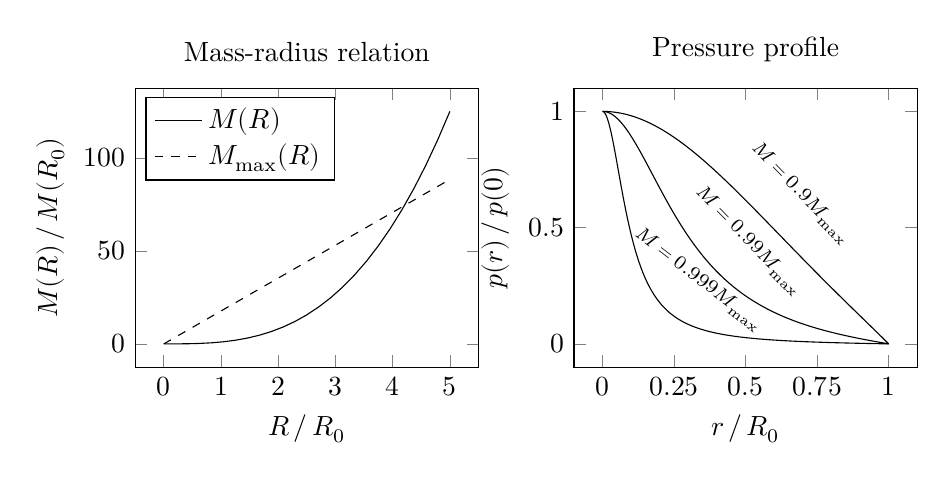
\begin{tikzpicture}[declare function={
		G = 1;
		M(\R,\E) = 4/3*pi*(\R)^3*\E;
		Mmax(\R) = 4*\R/(9*G);
		p(\r,\M,\R) = \M / (4/3*pi*(\R)^3) * (sqrt(1-2*G*\M*(\r)^2/(\R)^3) - sqrt(1-2*G*\M/(\R))) / (3*sqrt(1-2*G*\M/(\R)) - sqrt(1-2*G*\M*(\r)^2/(\R)^3));
	}]
		\begin{groupplot}[group style={group size=2 by 1, horizontal sep=0.1\textwidth}, width=0.49\textwidth]
		\nextgroupplot[
			title={\subcaption{\label{fig:incompressible_star:plot1}Mass-radius relation}},
			xlabel=$R \, / \, R_0$, ylabel=$M(R) \, / \, M(R_0)$, xtick distance=1, 
			legend pos=north west, legend cell align=left,
		]
		\pgfplotsinvokeforeach{0.006} {
			\addplot [domain=0:5, solid ] {M(x,#1) / M(1,#1)}; % node[pos=0.90, sloped, yshift=+6pt] {\scriptsize $\epsilon_0 = #1$};
			\addplot [domain=0:5, dashed] {Mmax(x) / M(1,#1)}; % node[pos=0.2, pin=above:{$M_\text{max}(R)$}] {};
		}
		\legend{$M(R)$, $M_\text{max}(R)$};
		\nextgroupplot[
			title={\subcaption{\label{fig:incompressible_star:plot2}Pressure profile}},
			xlabel=$r\, /\, R_0$, ylabel=$p(r) \, / \, p(0)$, xtick distance=0.25,
		]
		\pgfplotsinvokeforeach{0.9, 0.99, 0.999} {
			\addplot [domain=0:1,samples=200] {p(x,#1*Mmax(1),1)/p(0,#1*Mmax(1),1)} node[pos=0.54, sloped, yshift=+16pt] {\scriptsize $M = #1 M_\text{max}$};
		}
		\end{groupplot}
	\end{tikzpicture}
	\caption{
		\subref{fig:incompressible_star:plot1} Mass-radius relation $M(R) = 4 \pi R^3 \epsilon_0 / 3 c^2$ for a star of constant energy density $\epsilon_0$ compared to the maximum supported mass $M_\text{max}(R) = 4 c^2 R / 9 G$.
		\subref{fig:incompressible_star:plot2} Pressure profile $p(r)$ for stars of radius $R_0 = \sqrt{c^4 / G \epsilon_0}$ and masses $M$ approaching the limit $M_\text{max}(R_0)$.
	}
\end{figure}

\section{Weak-field limit and physical interpretation of mass}
\label{sec:weak_field_limit}

%TODO: move everything about interpretation of mass, energy density integral etc. to one section which has one thing in common: we look at the weak-field limit
%TODO: do weak-field limit of TOV equation, too

As we mentioned in \cref{sec:tov}, it is not apparent how to interpret the ``mass'' $M$ or ``energy'' $Mc^2$ in \cref{eq:einstein_to_tov:schwarzschild_mass}.
Here we will compare the results we have found so far to those of Newtonian gravity in the limit where particles move \emph{slowly} and the gravitational field is \emph{static} and \emph{weak}.

In Newtonian gravity, a particle is accelerated by the gravitational field
\begin{equation}
	\mathbf{g}(x) = - \nabla V(x) ,
	\label{eq:interpretation_m:newton2}
\end{equation}
where the gravitational potential $V$ is the solution to the Poisson equation
\begin{equation}
	\nabla^2 V(x) = 4 \pi G \rho(x) .
	\label{eq:interpretation_m:poisson}
\end{equation}

In general relativity, freely falling particles move along geodesics $x(\tau)$ that satisfy the \textbf{geodesic equation}
\begin{equation}
	\diff[2]{x^\mu}{\tau} + \Gamma^\mu_{\rho \sigma} \diff{x^\rho}{\tau} \diff{x^\sigma}{\tau} = 0 .
	\label{eq:geodesic}
\end{equation}
A \emph{slowly} moving particle has velocity $\diff{x^\mu}{\tau}$ with spatial component $\diff{x^i}{t} \ll c$ and is thus dominated by the spatial component $\diff{t}{\tau} \approx 1$.
Then $\diff{x^i}{\tau} \ll \diff{x^0}{\tau}$ and the geodesic equation can be approximated by
\begin{equation*}
	\diff[2]{x^\mu}{\tau} + \Gamma^\mu_{00} \, c^2 \left( \diff{t}{\tau} \right)^2 = 0 .
\end{equation*}
A \emph{static} field has $\partial_0 g\indices{_\mu_\nu} = 0$, so the Christoffel symbols \eqref{eq:def_christoffel} simplify to
\begin{equation*}
	\Gamma^\mu_{00} = \frac{1}{2} g\indices{^\mu^\lambda} (\partial_0 g\indices{_\lambda_0} + \partial_0 g\indices{_0_\lambda} - \partial_\lambda g\indices{_0_0}) = -\frac{1}{2} g\indices{^\mu^\lambda} \partial_\lambda g\indices{_0_0} .
\end{equation*}
A \emph{weak} gravitational field can be written as a perturbation 
\begin{equation}
	g\indices{_\mu_\nu} = \eta\indices{_\mu_\nu} + h\indices{_\mu_\nu}
	\quad \text{with} \quad
	\abs{h\indices{^\mu^\nu}} \ll 1
	\label{eq:weak_field_limit:metric_perturbation}
\end{equation}
on top of flat Minkowski space $\eta\indices{^\mu^\nu} = \text{diag}(-1, +1, +1, +1)$.
The inverse metric $g\indices{^\mu^\nu}$ should satisfy $g\indices{^\mu^\nu} g\indices{_\nu_\sigma} = \delta^\mu_\sigma$, so to first order in $h$ we must have
\begin{equation*}
	g\indices{^\mu^\nu} = \eta\indices{^\mu^\nu} - h\indices{^\mu^\nu} ,
\end{equation*}
where $h\indices{^\mu^\nu} = \eta\indices{^\mu^\rho} \eta\indices{^\nu^\sigma} h\indices{_\rho_\sigma}$ is raised with the Minkowski metric.
Calculating the relevant Christoffel symbols to first order in $h$, we find $\Gamma^\mu_{00} = -\frac{1}{2} \eta\indices{^\mu^\lambda} \partial_\lambda h\indices{_0_0}$, so the geodesic equation becomes
\begin{equation*}
	\diff[2]{x^\mu}{\tau} = \frac{1}{2} c^2 \eta\indices{^\mu^\lambda} \partial_\lambda h\indices{_0_0} \left( \diff{t}{\tau} \right)^2
	\quad \text{with spatial components} \quad
	\diff[2]{x^i}{t} = \frac{1}{2} c^2 \partial_i h\indices{_0_0} .
\end{equation*}
This is precisely \cref{eq:interpretation_m:newton2} if we identify $h\indices{_0_0} = -2V/c^2$ or $g\indices{_0_0} = -(1+2V/c^2)$, so a weak relativistic gravitational field $g\indices{_\mu_\nu} = \eta\indices{_\mu_\nu} + h\indices{_\mu_\nu}$ in fact describes Newtonian motion in the gravitational potential $V = -c^2 h\indices{_0_0} / 2$!
Moreover, the Schwarzschild metric has the element
\begin{equation}
	g\indices{_0_0} = - \left( 1 - \frac{2 G M}{r c^2} \right)
	\quad \text{with} \quad
	h\indices{_0_0} = 2GM/rc^2 ,
	\label{eq:weak_field_limit:schwarzschild_metric_tt}
\end{equation}
and $V = -c^2 h\indices{_0_0} / 2 = -G M / r$ is precisely the solution to Poisson's equation \eqref{eq:interpretation_m:poisson} for a spherical mass distribution, so general relativity does indeed describe Newtonian gravity in the weak-field limit!
In conclusion, this shows that it does make sense to interpret the Schwarzschild mass $M$ as the Newtonian mass of a star, as masses of distant stars are typically measured with results like Kepler's third law that follow from Newtonian gravity \cite[box 23.1]{ref:mtw}.

From the looks of \cref{eq:einstein_to_tov:schwarzschild_mass}, it is very tempting to also interpret $M c^2$ as the volume integral of the energy density over the star.
But $4 \pi r^2 \dif r$ is not a proper volume element.
In a proper spatial integral, the volume element should be $\sqrt{\abs{\gamma}} \dif^3 x = e^\beta r^2 \sin \theta \dif r \dif \theta \dif \phi$, where $\gamma\indices{_i_j} = g\indices{_i_j}$ is the spatial part of the metric and $\abs{\gamma}$ its determinant.
So the true volume integral of the energy density is really
\begin{equation*}
	\bar{M} c^2 = \integral{\epsilon(r) e^{\beta(r)} 4 \pi r^2}{r}{0}{R}.
\end{equation*}
The difference
\begin{equation*}
	\bar{M} c^2 - M c^2 = \integral{\epsilon(r) \left( \left( 1-\frac{2Gm}{rc^2} \right)^{-1/2} - 1 \right) 4 \pi r^2}{r}{0}{R} > 0
\end{equation*}
is in fact the binding energy that arises due to the gravitational attraction between the individual fluid elements in the star.
To see this, consider again the weak-field limit.
Comparing \cref{eq:weak_field_limit:metric_perturbation,eq:weak_field_limit:schwarzschild_metric_tt}, we see that we have the small parameter
\begin{equation}
	\frac{G m(r)}{rc^2} \ll 1 .
	\label{eq:weak_field_limit:small_gmr}
\end{equation}
Using the Taylor expansion $(1 - x)^{-1/2} = 1 + x/2$ and the mass-energy equivalence relation \eqref{eq:tov:mass_energy_equivalence}, we get
\begin{equation}
	\bar{M} c^2 - M c^2 \approx \integral{\frac{\epsilon(r)}{c^2} \frac{GM}{r} 4 \pi r^2}{r}{0}{R}
	                    =       \integral{\rho(r) \frac{GM}{r} 4 \pi r^2}{r}{0}{R} .
\end{equation}
As shown in \cite[exercise 23.7]{ref:mtw}, this is precisely the energy required to construct the star by sequentially placing thin shells of mass $\dif m = \rho(r) 4 \pi r^2 \dif r$ on top of each other, each subject to the gravitational attraction of the shells already placed below it.
This explains that $\bar{M} c^2 - M c^2$ is indeed the binding energy that would be required to disperse all the matter in the star to infinity.
% confusion about M, \bar{M}, resources:
% https://physics.stackexchange.com/q/196280/299916
% see MTW p. 602-, box at p. 603, p. 453
% see Schwarz p. 126

Finally, let us compare the TOV equation \eqref{eq:tov} and findings for relativistic incompressible stars from \cref{sec:incompressible_star} to those of Newtonian gravity.
To do so, we should first establish the Newtonian pressure gradient analogous to the relativistic one.

(TODO: figure for the below stuff)

Consider the mass element $\dif m = \rho(r) \dif A \dif r$ at distance $r$ from the center of a Newtonian star.
By Gauss' law it is attracted to the mass $m(r)$ inside the radius $r$ as if it were concentrated at the center, but experiences no attraction whatsoever from the remaining mass outside $r$ due to symmetry.
By Newton's law of gravity it is therefore pulled upon by the force
\begin{equation}
	\dif \mathbf{F}_1 = -\frac{G m(r) \dif m}{r^2} \hat{\textbf{r}} .
	\label{eq:weak_field_limit:force_newton}
\end{equation}
If the star is in hydrostatic equilibrium, this force must be exactly cancelled by the force
\begin{equation}
	\dif \textbf{F}_2 = - \Big( p(r + \dif r) - p(r) \Big) \dif A \, \hat{\textbf{r}} = -\dif p \dif A \, \hat{\textbf{r}}
	\label{eq:weak_field_limit:force_pressure}
\end{equation}
that arises from the pressure difference above and below the element.
Setting $\dif \textbf{F}_1 + \dif \textbf{F}_2 = 0$ then gives the \textbf{Newtonian pressure gradient}
\begin{equation}
	\diff{p}{r} = -\frac{G m(r) \rho(r)}{r^2} .
	\label{eq:weak_field_limit:newtonian_pressure_gradient}
\end{equation}

Solving this differential equation for a star of constant mass density $\rho(r) = \rho_0$ like we solved the TOV equation \eqref{eq:tov} in \cref{sec:incompressible_star}, we get the pressures
\begin{equation}
	p(r) = \frac{\rho_0}{2} \frac{G M}{R} \left( 1 + \frac{r}{R} \right) \left( 1 - \frac{r}{R} \right)
	\quad \text{and} \quad
	p(0) = \frac{\rho_0}{2} \frac{GM}{R} .
	\label{eq:weak_field_limit:newtonian_pressure}
\end{equation}
In this case, the pressure is well-behaved for all $r$.
This shows that Buchdal's theorem \eqref{eq:incompressible_star:buchdal} is a purely \emph{relativistic} result, and that no such limitation arises in Newtonian gravity!

% TODO: makes us suspect that Newton is taylor expansion of TOV
% TODO: check limit

Furthermore, we suspect that the relativistic pressure gradient \eqref{eq:tov} reduces to the Newtonian pressure gradient \eqref{eq:weak_field_limit:newtonian_pressure_gradient} in the Newtonian limit.
Comparing the two, we see that the relativistic equation indeed reduces to the Newtonian one if all the corrections to $1$ in the three parentheses vanish.
Let us see that this is actually the case.

First, note that by \cref{eq:weak_field_limit:small_gmr}, we have the small quantities
\begin{equation}
	\frac{Gm(r)}{rc^2} \ll 1
	\quad \text{and} \quad
	\frac{GM}{Rc^2} \ll 1 ,
	\label{eq:weak_field_limit:small3}
\end{equation}
so the rightmost correction in \cref{eq:tov} vanishes.

%By Taylor expanding the pressures \eqref{eq:incompressible_star:central_pressure} around the small parameter $GM/R \ll 1$, we get precisely the pressures in \cref{eq:weak_field_limit:newtonian_pressure}.
Second, we argued in \cref{sec:incompressible_star} that a star with constant energy density $\epsilon_0$ is the one that can withstand the most extreme pressure.
%We also deemed all physical stars to have a non-increasing energy density $\epsilon(r)$ away from the center.
A Taylor expansion of the relativistic central pressure \eqref{eq:incompressible_star:central_pressure} of an incompressible star in the limit \eqref{eq:weak_field_limit:small3} shows that it reduces precisely to the Newtonian central pressure $\epsilon_0 G M / 2 R c^2$ in \cref{eq:weak_field_limit:newtonian_pressure}.
Using this central pressure as an upper bound for \emph{all} stars, we expect that the pressure $p(r)$ and energy density $\epsilon(r)$ will always satisfy
\begin{equation}
	%\frac{p(r)}{\epsilon(r)} \leq \frac{p(0)}{\epsilon_0} = \frac{1}{2} \frac{GM}{Rc^2} \ll 1 .
	\frac{p(r)}{\epsilon(r)} \leq \frac{p(0)}{\epsilon(r)} 
	                         \leq \frac12 \frac{\epsilon(0)}{\epsilon(r)} \frac{GM}{Rc^2} \ll 1
	\qquad \text{(TODO: litt usikker på dette argumentet)}
	\label{eq:weak_field_limit:small1}
\end{equation}
by \cref{eq:weak_field_limit:small3}, provided that the energy density ratio $\epsilon(0) / \epsilon(r)$ is well-behaved.
To support this, we can argue that in a physical star, the speed of sound $v = c \sqrt{\difft{p}{\epsilon}}$ should not exceed $c$, so $\difft{p}{\epsilon} < 1$ and $p/\epsilon < 1$, denying the density ratio from diverging.
We saw that the incompressible star had $v = \infty$, but then we still have $\epsilon(0)/\epsilon(r) = 1$ and $p/\epsilon \ll 1$.
\Cref{eq:weak_field_limit:small1} causes the leftmost correction in \cref{eq:tov} to vanish, too.

Third, for a star with non-increasing energy density $\epsilon(r)$ away from the center $r=0$ -- which we deemed to be the only physical type of stars in \cref{sec:incompressible_star} -- we can pull the minimum density $\epsilon(r)$ outside the integral \eqref{eq:einstein_to_tov:m_integral} to get $m(r) c^2 \geq \frac{4}{3} \pi r^3 \epsilon(r)$, so
\begin{equation}
	\frac{4 \pi r^3 p(r)}{m(r) c^2} \leq \frac{4 \pi r^3 p(r)}{\frac{4}{3} \pi r^3 \epsilon(r)}
	                                =    \frac{3 p(r)}{\epsilon(r)}
						            \ll  1
	\label{eq:weak_field_limit:small2}
\end{equation}
by \cref{eq:weak_field_limit:small1}, and the middle correction in \cref{eq:tov} also vanishes.

Thus, we do indeed recover the Newtonian pressure gradient from the relativistic one in the Newtonian limit!
In fact, there is an alternative way to see it that requires much less work.
Written with mass density $\rho$ in place of energy density $\epsilon$, \cref{eq:tov} takes the form
\begin{equation}
	\diff{p}{r} = -\frac{G m(r) \rho(r)}{r^2} \left( 1 + \frac{p(r)}{\rho(r) c^2} \right) \left( 1 + \frac{4 \pi r^3 p(r)}{m(r) c^2} \right) \left( 1 - \frac{2 G m(r)}{r c^2} \right)^{-1} .
	\label{eq:tov_units}
\end{equation}
The Newtonian limit corresponds to sending $c \rightarrow \infty$, as this reduces the Lorentz transformations of relativity to the Galilei transformations of Newtonian physics.
But sending $c \rightarrow \infty$ kills all corrections in the three parentheses of \cref{eq:tov_units}, which restores the Newtonian pressure gradient \eqref{eq:weak_field_limit:newtonian_pressure_gradient}!

\appendix

\chapter{General relativity}
\label{chap:gr}

\textit{This appendix is inspired by references \cite{ref:carroll}, \cite{ref:mtw} and \cite{ref:mika_gr_notes}.}

\section{The geometry of curved spacetime}
\label{chap:gr_summary} % TODO: chap -> sec

\newcommand\pdvx[2]{\pdv{x^{#1}}{x^{#2}}}

In this section, we review the geometrical aspects of general relativity.
We make no attempt to be mathematically rigorous, but rather focus on listing important quantities and equations and the intuitive connection between them.
For more details, we refer to the references listed above which this summary is based on.

\subsection{Coordinates and tensors}

In general relativity, $3$-dimensional space and $1$-dimensional time are no longer regarded separate as they are in Newtonian mechanics.
They are rather intertwined into \emph{spacetime} -- a $(3+1)$-dimensional construct with \textbf{coordinates}
% position is just "coordinates", not a 4-vector: https://physics.stackexchange.com/questions/192886/does-spacetime-position-not-form-a-four-vector
\begin{equation}
	x^\mu = (x^0, x^1, x^2, x^3) .
\end{equation}
In flat Minkowski space, the coordinates could be taken as $x^\mu = (ct, x, y, z)$.
Mathematically, the geometry of spacetime is described by a \emph{Riemannian manifold} that generalizes flat Minkowski space to \emph{curved space}.
At every point on such a manifold, spacetime locally resembles Minkowski space in the \emph{tangent space} located at that point, and all such tangent spaces vary in a smooth manner from point to point.
For example, \cref{fig:tangent_space} pictures the tangent space at a point of the $2$-sphere manifold.
Familiar concepts like angles, lengths, area and volume apply locally in the tangent space at each point in infinitesimal form, and one can generalize such concepts to the full manifold by integrating the local contributions from one point on the manifold to another.

\begin{figure}
\centering
\includesvg[width=0.60\textwidth]{figures/tangent-space.svg}
\caption{\label{fig:tangent_space}The tangent space at a point on the $2$-sphere manifold can be pictured as the tangent plane at that point. If a vector field is placed on the manifold, the vector would lie in this tangent space. Illustration by \cite{ref:figure_tangent_space}.}
\end{figure}

% transformation law inspiration: https://math.stackexchange.com/a/958524 and Wikipedia: "holonomic basis"

\newcommand\lincombo[1]{\left( a \odv{#1}{\tau} + b \odv{#1}{\lambda} \right)}
\newcommand\lincomboslash[1]{\left( a \odv{#1}/{\tau} + b \odv{#1}/{\lambda} \right)}
We will place vector fields $V^\mu(x^\nu)$, and later tensor fields, that associate a vector $V^\mu$ to every point $x^\nu$ on a manifold.
As explained in \cref{fig:tangent_space}, such a vector lies in the tangent vector space at every point on the manifold.
To motivate the transformation properties of tensors on a manifold, we can use the fact that the set of directional derivatives constitute a vector space with basis vectors given by the partial derivatives. 
Suppose $\phi(x)$ is a scalar function and $x(\tau)$ and $x(\lambda)$ are two paths on the manifold with directional derivatives given through the chain rule as
\begin{equation}
	\odv{\phi}{\tau} = \odv{x^\mu}{\tau} \partial_\mu \phi
	\qquad \text{and} \qquad
	\odv{\phi}{\lambda} = \odv{x^\mu}{\lambda} \partial_\mu \phi .
\end{equation}
Then the linear combination $\lincomboslash{}$ is also a perfectly good derivative operator, as it is both linear and satisfies the product rule
\begin{equation}
	\lincombo{}(fg) = \ldots = \lincombo{f} g + \lincombo{g} f .
\end{equation}
One can verify that the set of all differential operators, implicitly assumed to work on some scalar function, satisfy all criteria for being a vector space.
Thus, like one can regard $\vec{V} = V^\mu \vec{e}_\mu$ as a vector with components $V^\mu$ and basis vectors $\vec{e}_\mu$, one can regard
\begin{equation}
	\odv{}{\lambda} = \odv{x^{\mu}}{\lambda} \partial_{\mu} 
\end{equation}
as a vector with components $\odv{x^{\mu}}/{\lambda}$ and basis vectors $\partial_\mu$.
To see this clearly, make a coordinate transformation
\begin{equation}
	x \rightarrow x'(x)
	\qquad \text{with inverse} \qquad
	x' \rightarrow x(x')
	\qquad \text{and Jacobians} \qquad
	\pdv{x'^{\alpha}}{x^\gamma} \pdv{x^{\gamma}}{x'^{\beta}} = \delta^{\alpha}_{\beta} .
	\label{eq:gr_summary:coordinate_transformation}
\end{equation}
Using the chain rule and the Jacobian property, the directional derivative transforms as
\begin{equation}
	\odv{}{\lambda} = \odv{x^{\mu'}}{\lambda} \partial_{\mu'} = \underbrace{\Bigg( \odv{x^{\alpha}}{\lambda} \pdvx{\mu'}{\alpha} \Bigg)}_\text{components} \underbrace{\Bigg( \pdvx{\beta}{\mu'} \partial_{\beta} \Bigg)}_\text{basis} = \odv{x^{\mu}}{\lambda} \partial_{\mu} .
\end{equation}
We see that the transformation of the components and the basis vectors exactly cancel each other, so the directional derivative is unchanged -- consistent with it being a vector.

Note that we adopted the convention $x^{\mu'} = x'^\mu$ of placing the prime on the \emph{index} rather than the underlying object, but defined to mean the same.
The benefit is that an index transforms with the partial derivative that has the primed coordinate in the \emph{same position as the index}, so we can always deduce the right transformation by simply staring at the expression.
%If there is a prime on an index, it means that a coordinate transformation has been applied to that index.
%The benefit of this is that an index transforms with the partial derivative that has the primed coordinate in the \emph{same position as the index} -- upper indices go with primed coordinates in the numerator, and lower indices with primes in the denominator.
%In addition, we are free to ``reuse'' the same index twice -- once as a free index, and once for the contraction.
%With this convention, we can always deduce the correct transformation laws from the index position, and we can place remaining indices so that they are contracted to yield an expression with the right number of free indices.

We define an $n$-dimensional \textbf{covariant vector} as an $n$-tuple $V_\mu$ that transforms with the \emph{same} matrix $\pdv{x^{\mu}}/{x^{\mu'}}$ as the change of basis as
\begin{subequations}
\begin{equation}
	V_{\mu'} = \pdv{x^{\mu}}{x^{\mu'}} V_\mu .
	\label{eq:covariant_transformation}
\end{equation}
Oppositely, we define an $n$-dimensional \textbf{contravariant vector} as an $n$-tuple $V^\mu$ that transforms with the \emph{inverse} matrix $\pdv{x^{\mu'}}/{x^{\mu}}$ as
\begin{equation}
	V^{\mu'} = \pdv{x^{\mu'}}{x^\mu} V_\mu .
	\label{eq:contravariant_transformation}
\end{equation}
More generally, we define a $n$-dimensional \textbf{tensor} of rank $(r,s)$ as an array composed of $r$ $n$-dimensional contravariant indices and $s$ $n$-dimensional covariant indices that transforms as
\begin{equation}
	T^{\mu_1' \dots \mu_r'}_{\nu_1' \dots \nu_s'} = \pdv{x^{\mu_1'}}{x^{\mu_1}} \cdots \pdv{x^{\mu_r'}}{x^{\mu_r}}
	                                                \pdv{x^{\nu_1}}{x^{\nu_1'}} \cdots \pdv{x^{\nu_s}}{x^{\nu_s'}}
												    T^{\mu_1 \dots \mu_r}_{\nu_1 \dots \nu_s}
	\label{eq:tensor_transformation}
\end{equation}
under the coordinate transformation \eqref{eq:gr_summary:coordinate_transformation}.
\end{subequations}

\iffalse
We will work with vector fields $V^\mu(x)$ on manifolds.
To each point on $x$ on the manifold, we associate a tangent vector $V^\mu(x)$.
How do vectors, and generally tensors, transform under a change of coordinates $x' = x'(x)$ on the manifold?
First, note that \emph{directional derivatives} constitute a vector space when acting on scalar functions.
Imagine two curves $x^\mu(\tau)$ and $x^\nu(\lambda)$ with directional derivatives $\odv{}/{\tau}$ and $\odv{}/{\lambda}$.
The linear combination $a \odv{}/{\tau} + b \odv{}/{\lambda}$ is also in the same space, as
\begin{equation}
	\lincombo{}(fg) = \ldots = \lincombo{f} g + \lincombo{g} f
\end{equation}
so the Leibniz rule is satisfied and the linear combination is also a proper derivative operator.
By the chain rule,
\begin{equation}
	\odv{}{\lambda} = \odv{x^\mu}{\lambda} \partial_\mu ,
\end{equation}
so the partial derivatives $\partial_\mu$ in fact constitute a natural basis for this vector space.
Since these are the basis vectors, we can deduce the transformation laws by requiring that $V^\mu \partial_\mu$ be constant under a change of coordinates:
\begin{equation}
	V^\mu \partial_\mu = V^{\mu'} \partial_{\mu'} = V^{\mu'} \pdv{x^\mu}{x^{\mu'}} \partial_\mu ,
\end{equation}
so the general \textbf{transformation law for contravariant vectors} is
\begin{equation}
	V^{\mu'} = \pdv{x^{\mu'}}{x^\mu} V_\mu .
\end{equation}

To get the transformation law for covariant vectors, we make use of the gradient of a scalar function
\begin{equation}
	\nabla \phi = \partial_\mu \phi \vec{e}^\mu 
\end{equation}
Using the chain rule,
\begin{equation}	
	\partial_{\mu'} \phi = \pdv{x^\mu}{x^{\mu'}} \partial_\mu \phi ,
\end{equation}
so the \textbf{transformation law for covariant vectors} is
\begin{equation}
	V_{\mu'} = \pdv{x^{\mu}}{x^{\mu'}} V_\mu .
\end{equation}
This line of reasoning can be extended to find the \textbf{general transformation law for tensors} (where we suppress the ordering of the indices)
\begin{equation}
	T^{\mu_1' \dots \mu_m'}_{\nu_1' \dots \nu_n'} = \pdv{x^{\mu_1'}}{x^{\mu_1}} \cdots \pdv{x^{\mu_m'}}{x^{\mu_m}}
	                                                \pdv{x^{\nu_1'}}{x^{\nu_1}} \cdots \pdv{x^{\nu_n'}}{x^{\nu_n}}
												    T^{\mu_1 \dots \mu_m}_{\nu_1 \dots \nu_n}
\end{equation}
\fi

\subsection{Metric tensor}

The \textbf{metric tensor}
\begin{equation}
	g\indices{_\mu_\nu}(x) = \vec{e}_\mu(x) \cdot \vec{e}_\nu(x)
\end{equation}
is defined as the inner products between basis vectors $\vec{e}_\mu$ that span the tangent spaces at each point $x$ on the manifold.
It thus encodes the lengths vectors of the basis vectors and angles between them and is a fundamental object that describes the geometry of the manifold.

We define the \textbf{inverse metric tensor} $g^{\mu \nu}$ as the inverse matrix satisfying
\begin{equation}
	g^{\mu \nu} g_{\nu \sigma} = \delta^\mu_\sigma .
\end{equation}
Using the metric and its inverse, we can \textbf{raise and lower indices} on tensors.
For example, the object $g_{\mu \nu} V^\nu$, according to definition \eqref{eq:tensor_transformation}, transforms as a covariant vector
\begin{equation}
	g_{\mu' \nu'} V^{\nu'} = \left( \pdvx{\alpha}{\mu'} \pdvx{\beta}{\nu'} g_{\alpha \beta} \right) \left( \pdvx{\nu'}{\nu} V^{\nu} \right) = \pdvx{\alpha}{\mu'} g_{\alpha \nu} V^\nu ,
\end{equation}
so it is meaningful to label it as a covariant vector with a lower index $V_\mu = g_{\mu \nu} V^\nu$.
Similarly, we can use the inverse metric $g^{\mu \nu}$ to raise indices.
As this argument only relied on the defining transformation law \eqref{eq:tensor_transformation}, it is clear that any tensor of rank $(2,0)$ or $(0,2)$ would suffice to raise or lower indices.
But the metric is the most natural choice, as it is inherent to the manifold and always available to us.

\subsection{Line element and volume}

From the metric tensor, one defines the \textbf{line element}
\begin{subequations}
\begin{equation}
	\dif s = \sqrt{g\indices{_\mu_\nu} \dif x^\mu \dif x^\nu}
	\label{eq:def_line_elem}
\end{equation} 
that extends the concept of distance locally to every point on the manifold.
By integrating the line element from one point on the manifold to another, one can compute the total distance
\begin{equation}
	s = \int_1^2 \dif s = \int_1^2 \sqrt{g\indices{_\mu_\nu} \dif x^\mu \dif x^\nu}
\end{equation}
between the points.
Similarly, one can compute the \textbf{volume} of a region
\begin{equation}
	V = \int \dif V = \int \sqrt{-\det{\gamma}} \dif x^1 \dif x^2 \dif x^3 ,
\end{equation}
\end{subequations}
where $\gamma$ is the induced metric on the surface and $\det{\gamma} < 0$ its determinant.
The factor $\sqrt{-\det{\gamma}}$ arises to make the volume element $\dif^n x \sqrt{-\det{\gamma}}$ invariant under coordinate transformations.

\subsection{Covariant derivatives and connection coefficients}

Knowing how vectors and general tensors transform, let us generalize the notion of a derivative to curved space.
By the transformation rules we have found so far, the normal partial derivative of a vector transforms as
\begin{equation}
	\partial_{\mu'} V^{\nu'} = \bigg( \pdvx{\mu}{\mu'} \partial_\mu \bigg) \bigg( \pdvx{\nu'}{\nu} V^\nu \bigg)
	                         = \pdvx{\mu}{\mu'} \pdvx{\nu'}{\nu} \partial_\mu V^\nu + \pdvx{\mu}{\mu'} \pdv{x^{\nu'}}{x^\mu, x^\nu} V^\nu .
\end{equation}
The first term respects the tensor transformation law \eqref{eq:tensor_transformation}, but the second does not, so $\partial_\mu V^\nu$ is \emph{not} a tensor.
We define a tensorial derivative $\nabla_\mu$ that by demanding that it transforms as
\begin{equation}
	\nabla_{\mu'} V^{\nu'} = \pdvx{\mu}{\mu'} \pdvx{\nu'}{\nu} \nabla_\mu V^\nu .
\label{eq:gr_summary:covariant_derivative_demand}
\end{equation}
It turns out that our requirements can be met if we define the \textbf{covariant derivative} as
\begin{equation}
	\nabla_\mu V^\nu = \partial_\mu V^\nu + \Gamma_{\sigma \mu}^\nu V^\sigma .
	%\qquad \text{or} \qquad
	%\nabla_\mu V_\nu = \partial_\mu V_\nu - \Gamma_{\nu \mu}^\sigma V_\sigma ,
\end{equation}
It is possible to show that it obeys the tensorial transformation \eqref{eq:gr_summary:covariant_derivative_demand} if the so-called \textbf{connection coefficients} $\Gamma_{\sigma _\mu}^\nu$ transform according to \cite[equation 3.6-3.10]{ref:carroll} 
\begin{equation}
	\Gamma^{\nu'}_{\mu' \lambda'} = \pdvx{\mu}{\mu'} \pdvx{\lambda}{\lambda'} \pdvx{\nu'}{\nu}  \Gamma^{\nu}_{\mu \lambda} + \pdvx{\mu}{\mu'} \pdvx{\lambda}{\lambda'} \pdv{x^{\nu'}}{x^\mu, x^\lambda} .
	\label{eq:connection_transformation}
\end{equation}
It is possible to generalize the covariant derivative to an arbitrary tensor $T^{\alpha_1 \ldots \alpha_r}_{\beta_1 \ldots \beta_s}$ of rank $(r,s)$ (where we suppress the order of the indices) by adding more terms with connection coefficients.
The general \textbf{covariant derivative} that respects the tensorial transformation law \eqref{eq:tensor_transformation} turns out to be \cite[equation 3.11-3.16]{ref:carroll}
\begin{equation}
\begin{split}
	\nabla_\mu T^{\alpha_1 \ldots \alpha_r}_{\beta_1 \ldots \beta_s} &= \partial_\mu T^{\alpha_1 \ldots \alpha_r}_{\beta_1 \ldots \beta_s} \\
	                                                                 &+ \Gamma^{\alpha_1}_{\sigma\mu} T^{\sigma \alpha_2 \ldots \alpha_r}_{\beta_1 \ldots \beta_s} + \dots + \Gamma^{\alpha_r}_{\sigma\mu} T^{\alpha_1 \ldots \alpha_{r-1}\sigma}_{\beta_1 \ldots \beta_s} \\
	                                                                 &- \Gamma^\sigma_{\beta_1 \mu} T^{\alpha_1 \ldots \alpha_r}_{\sigma \beta_2 \ldots \beta_s} - \cdots - \Gamma^\sigma_{\beta_s \mu} T^{\alpha_1 \ldots \alpha_r}_{\beta_1 \ldots \beta_{s-1} \sigma} .
	\label{eq:def_cov_deriv}
\end{split}
\end{equation}
That is, for each upper index $\alpha_i$, add $+\Gamma^{\alpha_i}_{\sigma \mu} T^{\alpha_1 \ldots \alpha_{i-1} \sigma \alpha_{i+1} \ldots \alpha_r}_{\beta_1 \ldots \beta_s}$,
and for each lower index $\beta_i$, add $-\Gamma^{\sigma}_{\beta_i \mu} T^{\alpha_1 \ldots \alpha_r}_{\beta_1 \ldots \beta_{i-1} \sigma \beta_{i+1} \ldots \beta_s}$,

Note that the connection coefficients \eqref{eq:connection_transformation} \emph{do not} transform like tensors -- the whole point is to stash the non-tensorial behavior into the connection coefficients so that the \emph{covariant derivative} transforms as a tensor.
However, since $\nabla_\mu V^\nu$ and $\hat{\nabla}_\mu V^\nu$ for two different connection coefficients $\Gamma^\alpha_{\beta \mu}$ and $\hat{\Gamma}^\alpha_{\beta \mu}$ by definition are tensors, the \emph{difference}
\begin{equation}
	S\indices{^\alpha_\beta_\gamma} = \Gamma^\alpha_{\beta \gamma} - \hat{\Gamma}^\alpha_{\beta \gamma}
\end{equation}
between two connection coefficients \emph{does} transform like a tensor.

There are many possible choices of the connection coefficients that satisfy \cref{eq:connection_transformation}.
However, it turns out that we can find a set of \emph{unique} connection coefficients from the \emph{metric} if we impose two additional requirements.
First, we demand that the \textbf{torsion tensor}
\begin{equation}
	T\indices{^\alpha_\beta_\gamma} = \Gamma^\alpha_{\beta\gamma} - \Gamma^\alpha_{\gamma\beta}
	\label{eq:torsion_tensor}
\end{equation}
vanishes.
Equivalently, the connection coefficients $ \Gamma^\alpha_{\beta\gamma} = \Gamma^\alpha_{\beta\gamma} $ are symmetric in the lower indices.
Second, we require \textbf{metric compatibility}
\begin{equation}
	\nabla_\rho g_{\mu \nu} = 0 ,
\end{equation}
expressing that the metric is covariantly constant.
One can show that this guarantees that lengths of vectors and angles between them are preserved under parallel transport, which we will study in the next section, making this a reasonable demand \cite[equation 2.10]{ref:hehl}.
The covariantly constant nature of the metric implies that we can view spacetime as a continuum of flat Minkowski spacetimes, sewn together by the connection $\Gamma^\alpha_{\beta \gamma}$.
Metric compatibility implies that
\begin{equation}
	g_{\mu \lambda} \nabla_\rho V^\lambda = \nabla_\rho (g_{\mu \lambda} V^\lambda) = \nabla_\rho V_\mu ,
\end{equation}
so we can raise and lower indices inside covariant derivatives, even if the metric is outside.
Using both of these assumptions, we can write out three metric compatibility requirements
\newcommand\metriccompatibilityequation[3]{\nabla_{#1} g_{{#2}{#3}} &= \partial_{#1} g_{{#2}{#3}} - \Gamma^\lambda_{{#1}{#2}} g_{\lambda {#3}} - \Gamma^\lambda_{{#1}{#3}} g_{{#2} \lambda} = 0}
\begin{subequations}
\begin{align}
	\metriccompatibilityequation{\rho}{\mu}{\nu} , \\
	\metriccompatibilityequation{\mu}{\nu}{\rho} , \\
	\metriccompatibilityequation{\nu}{\rho}{\mu} .
\end{align}
\end{subequations}
By subtracting the second and third equation from the first and solving the resulting equation for the connection, we find the \textbf{Christoffel symbols} or \textbf{metric connection}
\begin{equation}
	\Gamma^\sigma_{\mu \nu} = \frac{1}{2} g\indices{^\sigma^\rho} \left(
		\partial\indices{_\mu} g\indices{_\nu_\rho} +
		\partial\indices{_\nu} g\indices{_\rho_\mu} -
		\partial\indices{_\rho} g\indices{_\mu_\nu}
	\right) .
	\label{eq:def_christoffel}
\end{equation}
In general relativity, we will \emph{always} use this unique representation of the connection coefficients given in terms of the metric only.
With this choice, the metric single-handedly determines the geometry of spacetime, as it is the only fundamental object that all the other geometric quantities we have looked at depends on.
In fact, the requirements of zero torsion and metric compatibility that led to this metric can be viewed as defining features of general relativity.
By relaxing either of these requirements, one can come up with various generalizations of general relativity.
For example, by allowing for nonzero torsion \eqref{eq:torsion_tensor}, one obtains the \emph{Einstein-Cartan theory} of gravitation.
One can show that the inclusion of torsion is equivalent to accounting for the \emph{spin} of the microscopic particles that make up the macroscopic matter \cite{ref:hehl}.
However, general relativity is concerned with describing \emph{macroscopic} objects, which justifies our demand of zero torsion.

\iffalse
\begin{align}
	\nabla_c T\indices{^{a_1 \ldots a_r}_{b_1 \ldots b_s}} &= \partial_c {T^{a_1 \ldots a_r}}_{b_1 \ldots b_s} \\
	                                                       &+ \Gamma^{a_1}_{dc} T\indices{^{d a_2 \ldots a_r}_{b_1 \ldots b_s}} + \dots + \Gamma^{a_r}_{dc} T\indices{^{a_1 \ldots a_{r-1}d}_{b_1 \ldots b_s}} \\
	                                                       &- {\Gamma^d}_{b_1 c} {T^{a_1 \ldots a_r}}_{d b_2 \ldots b_s} - \cdots - {\Gamma^d}_{b_s c} {T^{a_1 \ldots a_r}}_{b_1 \ldots b_{s-1} d}.
	\label{eq:def_cov_deriv}
\end{align}
\fi

\subsection{Parallel transport and geodesic equation}
\label{sec:geodesic}

\begin{figure}
\centering
\includesvg[width=0.5\textwidth]{figures/parallel_transport.svg}
\caption{\label{fig:parallel_transport}When a vector is parallel transported around a closed loop on the $2$-sphere, its final direction depends on the path taken. Illustration by \cite{ref:figure_parallel_transport}.}
\end{figure}

Now that we know how to take proper derivatives of vector fields and general tensor fields on manifolds, we can discuss how to parallel transport vectors on the manifold.
In flat space, we can move a vector around and keep its Cartesian components constant to parallel transport it.
But on a curved $2$-sphere, a vector that is parallel transported will end up being different depending on the route taken, as illustrated in \cref{fig:parallel_transport}.
Generalizing the directional derivative $\odv{}/{\tau} = (\odv{x^\mu}/{\tau}) \partial_\mu$ from calculus, we define the \textbf{directional covariant derivative} along a path $x(\tau)$ as
\begin{equation}
	\frac{D}{\mathrm{d} \tau} = \odv{x^\mu}{\tau} \nabla_\mu,
\end{equation}
where $\nabla_\mu$ is the covariant derivative \eqref{eq:def_cov_deriv}.
We say that a tensor is parallel transported if its components are kept constant during transport, as expressed by
\begin{equation}
	\frac{D}{\mathrm{d} \tau} T^{\mu_1 \ldots \mu_m}_{\nu_1 \ldots \nu_n} = 0 .
\end{equation}
For the special case of a vector $V^\mu$ we get the \textbf{equation of parallel transport}
\begin{equation}
	\odv{V^\mu}{\tau} + \Gamma^{\mu}_{\sigma \rho} \odv{x^\sigma}{\tau} V^\rho = 0 .
	\label{eq:parallel_transport}
\end{equation}
The solution of this first-order differential equation is the continuation $V^\mu(\tau)$ from an initial vector $V^\mu(0)$ along the path such that its components are constant.

In Euclidean space, a straight line is the shortest path between two points.
In curved space, we call the shortest path between two points on a manifold a \textbf{geodesic}.
An equivalent definition of both a straight line and a geodesic is that it is the path $x(\tau)$ that parallel transports its own tangent vector $\odv{x^\mu}/{\tau}$.
Inserted into the equation of parallel transport \eqref{eq:parallel_transport}, we find the \textbf{geodesic equation}
\begin{equation}
	\odv[2]{x^\mu}{\tau} + \Gamma^\mu_{\rho \sigma} \odv{x^\rho}{\tau} \odv{x^\sigma}{\tau} = 0 .
	\label{eq:geodesic}
\end{equation}
In flat spacetime, it reduces to the equation of a straight line $\odv[2]{x^\mu}/{\tau} = 0$.
One of Einstein's profound insights of general relativity was that gravity does not simply alter the path of a freely falling particle away from the straight line it would follow in Euclidean space in the absence of gravity.
Instead, gravity presents itself in the geometry of spacetime, as the presence of energy-momentum curves spacetime and lays geodesic ``tracks'' according to \cref{eq:geodesic} that any freely falling particle is destined to follow.
\emph{Gravity is geometry}.

\subsection{Riemann curvature tensor, Ricci tensor and Ricci scalar}

% motivate by connecting it to the metric? 
% https://math.stackexchange.com/a/1213124 
% https://math.stackexchange.com/q/884794 
% https://math.stackexchange.com/q/2896648
% https://en.wikipedia.org/wiki/Ricci_curvature#Direct_geometric_meaning (taylor expansion around normal coords) 

So far we have used the term ``curvature'' quite informally -- let us now formalize this.
We already saw that parallel transporting a vector along different paths on a curved manifold like the $2$-sphere yield different results.
We have also seen that the covariant derivative measures the rate of change of a vector along some direction compared to what it would've been if it was parallel transported.
Thus, the commutator $[ \nabla_\mu, \nabla_\nu ] V^\rho = \nabla_\mu V^\rho - \nabla_\nu V^\rho$ measures the difference of parallel transporting a vector along the two different directions.
Using \cref{eq:def_cov_deriv}, it turns out we can write this as
\begin{equation}
	[ \nabla_\mu, \nabla_\nu ] V^\rho = R\indices{^\rho_{\sigma \mu \nu}} V^\sigma - T\indices{^\lambda_{\mu \nu}} \nabla_\lambda V^\rho ,
\end{equation}
where $T\indices{^\lambda_{\mu \nu}}$ is the torsion tensor \eqref{eq:torsion_tensor} that we assume to vanish and we define the \textbf{Riemann curvature tensor}
\begin{equation}
	R\indices{^\rho_\sigma_\mu_\nu} =
	\partial\indices{_\mu} \Gamma^\rho_{\nu \sigma} -
	\partial\indices{_\nu} \Gamma^{\rho}_{\mu \sigma} +
	\Gamma^\rho_{\mu \lambda} \Gamma^{\lambda}_{\nu \sigma} -
	\Gamma^\rho_{\nu \lambda} \Gamma^{\lambda}_{\mu \sigma} .
	\label{eq:def_riemann_tensor}
\end{equation}
We expect that if space is flat, then a parallel transported vector should not depend on the path, so the commutator and thus the Riemann tensor should vanish.
If there exists \emph{any} choice of coordinates in which the curvature tensor vanishes, then it vanishes in \emph{all} coordinates by its tensorial nature, and this is our ultimate definition of \textbf{flat space}.
In fact, it turns out that at any point $x_0$ we can find \textbf{normal coordinates} $x^\mu$ in which the metric locally resembles Minkowski space with $g_{\mu \nu} = \eta_{\mu \nu}$ and $\partial_\sigma g_{\mu \nu} = 0$ to first order in the displacement.
To second order in the displacement, \cite{ref:metric_taylor_expansion} shows that the metric can be written
\begin{equation}
	g_{\mu \nu}(x) = \eta_{\mu \nu} - \frac12 R_{\alpha \mu \beta \nu} (x^\alpha - x_0^\alpha) (x^\beta - x_0^\beta) .
\end{equation}
This shows that the Riemann tensor is a \emph{very} appropriate measure of curvature.
Moreover, \textbf{Einstein's equivalence principle} and the related \textbf{principle of general covariance} states that a physical law that is expressed by a tensor equation in Minkowski space \emph{also} holds in any reference frame in the presence of gravity. \cite[chapter 4]{ref:weinberg_gravity}

% TODO: motivate
% https://en.wikipedia.org/wiki/Introduction_to_the_mathematics_of_general_relativity#Curvature_tensor (need two indices to enter the Einstein field equations -- "geometry" = metric comes with 2 indices, and "energy-momentum" come with 2 indices, https://physics.stackexchange.com/a/220650)
% see great motivation at https://physics.stackexchange.com/a/220650
% and great motivation at https://physics.stackexchange.com/a/219682

From the curvature tensor, we can form tensors of lower rank by contracting some of its indices.
We know that the energy-momentum tensor $T^{\mu \nu}$ that enter the Einstein field equations \eqref{eq:einstein} are of second rank, so if it is to determine the curvature of spacetime by a tensor equation, then the curvature tensor must be contracted to form a tensor of equal rank.
With the Christoffel connection \cref{eq:def_christoffel}, it turns out that the only independent contraction we can make is the \textbf{Ricci tensor}
\begin{equation}
	R\indices{_\mu_\nu} = R\indices{^\lambda_\mu_\lambda_\nu} .
	\label{eq:def_ricci_tensor}
\end{equation}
The two other possible contractions either vanish or are related to the Ricci tensor.
Thus, the simplest scalar quantity we can form that represents curvature is the \textbf{Ricci scalar}
\begin{equation}
	R = R\indices{^\mu_\mu} .
	\label{eq:def_ricci_scalar}
\end{equation}



\section{Least-action derivation of the Einstein field equations}
\label{sec:einstein_derivation}

Following \cite[section 4.3]{ref:carroll}, we will derive the Einstein field equations
\begin{equation}
	R_{\mu \nu} - \frac{1}{2} R g_{\mu \nu} = \frac{8 \pi G}{c^4} T_{\mu \nu}
\end{equation}
from the principle of least action.
We will \emph{postulate} the action
\begin{equation}
	S[g_{\mu \nu}, \nabla_\sigma g_{\mu \nu}] = \int \dif^n x \lagr(g_{\mu \nu}, \nabla_\sigma g_{\mu \nu})
	                                          = \int \dif^n x \sqrt{-\det{g}} \hat{\lagr}(g_{\mu \nu}, \nabla_\sigma g_{\mu \nu})
\end{equation}
that, when varied with respect to the metric $g_{\mu \nu}$ and subject to the principle of least action $\variation{S} = 0$, yields the Einstein field equations.
Here $\lagr$ and $\hat{\lagr}$ are Lagrangian densities with and without the metric determinant $\det{g} < 0$.
As the strategy simply involves \emph{guessing} the correct action that produces the desired equations, this derivation is not based on any physical first principles, so its consequences would ultimately have to be experimentally verified.
Nevertheless, \cite[page 160-161]{ref:carroll} explains how one can at the very least narrow down the choice of action based on scalar quantities that are relevant for describing curved space.

We postulate the \textbf{Hilbert action}
\begin{equation}
	% i have x = (ct, x1, x2, x3), so I have a c "already" in the first component
	% this is normal! see e.g. https://physics.stackexchange.com/a/322055/299916
	% remember [R] = 1/m^2
	S_H = \frac{c^3}{16 \pi G} \int \dif^n x \sqrt{-\det{g}} \, R .
	\label{eq:einstein_derivation:hilbert_action}
\end{equation}
As the Lagrangian is a scalar quantity and we showed that the simplest scalar quantity we could create is the Ricci scalar \eqref{eq:def_ricci_scalar}, it is not an unreasonable guess.
The prefactor has been conveniently chosen to yield correct result \eqref{eq:einstein_derivation:einstein_matter} in the end, which we saw in \cref{sec:einstein_to_poisson} led to Newtonian gravity in the Newtonian limit.
From an ignorant point of view, we could instead regard it as an arbitrary constant at this point, and eventually replace it with the right combination of constants that reproduce Newtonian gravity in the Newtonian limit.
We could get the corresponding equations of motion by plugging the Lagrangian density $\hat{\lagr} = R c^3 / 16 \pi G$ into the Euler-Lagrange equations
\begin{equation}
	\pdv{\hat{\lagr}}{\phi} - \nabla_\mu \left( \pdv{\hat{\lagr}}{{\left(\nabla_\mu \phi\right)}} \right) = 0 .
\end{equation}
In fact Hilbert himself did this \cite{ref:hilbert_from_lagrange}, but doing so requires a great deal of effort.
Instead, we will vary the action with respect to the metric and express the variation in the form 
\begin{equation}
	\variation{S_H} = \int \dif^n x \sqrt{-\det{g}} F(g_{\mu \nu}, \nabla_\sigma g_{\mu \nu}) \, \variation{g^{\mu \nu}} = 0 .
	\label{eq:einstein_derivation:action_form}
\end{equation}
Then we can conclude that the equations of motion are $F(g_{\mu \nu}, \nabla_\sigma g_{\mu \nu}) = 0$.

It may sound more natural to express the variation in terms of the ordinary metric $g_{\mu \nu}$ instead of its inverse $g^{\mu \nu}$, like we did above.
But since $g^{\mu \lambda} g_{\lambda \nu} = \delta^\mu_\nu$, varying both sides with the product rule relates the two by
\begin{equation}
	\variation{g_{\mu \nu}} = -g_{\mu \rho} g_{\nu \sigma} \variation{g^{\rho \sigma}} .
	\label{eq:einstein_derivation:var_g_ginv}
\end{equation}
Thus, the stationary points are the same regardless of which one we vary with respect to.
We vary with respect to the inverse metric, as it makes the derivation flow more naturally.

Using $R = R\indices{^\mu_\mu} = g^{\mu \nu} R_{\mu \nu}$ and varying the action \eqref{eq:einstein_derivation:hilbert_action} with the product rule, we obtain
\begin{equation}
	\variation{S_H} = \frac{c^3}{16 \pi G} \left(
	                  \underbrace{\int \dif^n x \sqrt{-\det{g}} \, g^{\mu \nu} \variation{R_{\mu \nu}}}_{\textstyle \variation{S}_1}
	                + \underbrace{\int \dif^n x \sqrt{-\det{g}} \, R_{\mu \nu} \variation{g^{\mu \nu}}}_{\textstyle \variation{S}_2}
	                + \underbrace{\int \dif^n x \, R \, \variation{\sqrt{-\det{g}}}                      }_{\textstyle \variation{S}_3}
					\right) .
%\begin{split}
%	                                                                                               \variation{S}_1 &= \int \dif^n x \sqrt{-\det{g}} g^{\mu \nu} \variation{R_{\mu \nu}} \\
%	\variation{S} = \variation{S}_1 + \variation{S}_2 + \variation{S}_3 , \quad \text{where} \quad \variation{S}_2 &= \int \dif^n x \sqrt{-\det{g}} R_{\mu \nu} \variation{g^{\mu \nu}} \\
%	                                                                                               \variation{S}_3 &= \int \dif^n x R \variation{\sqrt{-\det{g}}} \\
%\end{split}
%\begin{split}
%	\variation{S} &= \int \dif^n x \sqrt{-\det{g}} g^{\mu \nu} \variation{R_{\mu \nu}} \\
%	              &+ \int \dif^n x \sqrt{-\det{g}} R_{\mu \nu} \variation{g^{\mu \nu}} \\
%	              &+ \int \dif^n x R \variation{\sqrt{-\det{g}}} \\
%\end{split}
	\label{eq:einstein_derivation:ds_split}
\end{equation}
The second term $\variation{S}_2$ is already in the desired form \eqref{eq:einstein_derivation:action_form}, but we must do some work to bring $\variation{S}_1$ and $\variation{S}_3$ to the same form.

% TODO: latex package glossary?

First, let us take care of $\variation{S}_1$ by reexpressing $\variation{R_{\mu \nu}}$ in terms of metric variations in a top-down manner.
The Ricci tensor $R_{\mu \nu} = R\indices{^\lambda_\mu_\lambda_\nu}$ is the contraction of the Riemann tensor \eqref{eq:def_riemann_tensor}.
Varying it, we get
% TODO: do more intelligently by writing (\mu <-> \nu), etc.
\begin{equation}
	\variation{R\indices{^\rho_\sigma_\mu_\nu}} = \partial_\mu \variation{\Gamma^\rho_{\nu \sigma}}
	                                            - \partial_\nu \variation{\Gamma^\rho_{\mu \sigma}}
												+ \left(\variation{\Gamma^\rho_{\mu \lambda}}\right) \Gamma^\lambda_{\nu \sigma}
												+ \Gamma^\rho_{\mu \lambda} \left(\variation{\Gamma^\lambda_{\nu \sigma}\right)}
												- \left(\variation{\Gamma^\rho_{\nu \lambda}}\right) \Gamma^\lambda_{\mu \sigma}
												- \Gamma^\rho_{\nu \lambda} \left(\variation{\Gamma^\lambda_{\mu \sigma}\right)} .
	\label{eq:einstein_derivation:var_riemann}
\end{equation}
Now reexpress the variations of the Christoffel symbols.
Instead of hammering straight through their definition \eqref{eq:def_christoffel}, we observe that while single Christoffel symbols do not transform as a tensor, their \emph{variation} is the difference between two Christoffel symbols and \emph{do} \cite[page 96,98]{ref:carroll}.
It is therefore meaningful to use \cref{eq:def_cov_deriv} to take its covariant derivative
\begin{equation}
	\nabla_\lambda \variation{\Gamma^\rho_{\nu \mu}} = \partial_\lambda \variation{\Gamma^\rho_{\nu \mu}} 
	                                                 + \Gamma^\rho_{\lambda \sigma} \variation{\Gamma{^\sigma_{\nu \mu}}} 
	                                                 - \Gamma^\sigma_{\lambda \nu} \variation{\Gamma{^\rho_{\sigma \mu}}} 
	                                                 - \Gamma^\sigma_{\lambda \mu} \variation{\Gamma{^\rho_{\nu \sigma}}} .
	\label{eq:einstein_derivation:christoffel_cov_deriv}
\end{equation}
Flipping this equation around for $\partial_\lambda \variation{\Gamma^\rho_{\nu \mu}}$ and substituting the result into the variation of the Riemann tensor \eqref{eq:einstein_derivation:var_riemann}, we witness an avalanche of cancellations, leaving only the terms
\begin{equation}
	\variation{R\indices{^\rho_\mu_\lambda_\nu}} = \nabla_\lambda \variation{\Gamma^\rho_{\nu \mu}}
	                                             - \nabla_\nu \variation{\Gamma^\rho_{\lambda \mu}} .
\end{equation}
The variation of the Ricci tensor follows by contracting $\rho$ and $\lambda$. 
Then the first term in the variation of the action becomes
\begin{equation}
\begin{split}
	\variation{S}_1 &= \int \dif^n x \sqrt{-\det{g}} \, g^{\mu \nu} \left( \nabla_\lambda \variation{\Gamma^\lambda_{\mu \nu}} - \nabla_\nu \variation{\Gamma^\lambda_{\lambda \mu}} \right) \\
	                &= \int \dif^n x \sqrt{-\det{g}} \, \nabla_\sigma \left( g^{\mu \nu} \variation{\Gamma^\sigma_{\mu \nu}} - g^{\mu \sigma} \variation{\Gamma^\lambda_{\lambda \mu}} \right) . \\
	\label{eq:einstein_derivation:ds1_intermediate}
\end{split}
\end{equation}
We still have not brought the variation to the form \eqref{eq:einstein_derivation:action_form}, but it does not matter.
By \textbf{Stokes theorem} \cite[equation 3.35]{ref:carroll}
\begin{equation}
	\int_M \dif^n x \sqrt{\abs{g}} \nabla_\mu V^\mu = \int_{\partial M} \dif^{n-1} \sqrt{\abs{\gamma}} n_\mu V^\mu ,
\end{equation}
our integral for $\variation{S}_1$ over $n$-space can be converted into a boundary integral over $(n-1)$-space at infinity.
But the variational method that we have used here asserts that there is no variation on the boundary, so
\begin{equation}
	\variation{S}_1 = 0 .
\end{equation}

Let us now express $\variation{S}_3$ in terms of $\variation{g^{\mu \nu}}$.
We will need the matrix identity
\begin{equation}
	\log \, \det{M} = \trace \log M  .
	\label{eq:matrix_log_det_trace}
\end{equation}
This is trivial for diagonal matrices $M$.
By using the property $\det{AB} = \det{A} \det{B}$, we can easily extend it to diagonalizable matrices $M = P D P^{-1}$.
Varying both sides of \cref{eq:matrix_log_det_trace}, we obtain \cite{ref:matrix_ln_det_tr_exercise}
\begin{equation}
	\frac{\variation{\det{M}}}{\det{M}} = \trace(M^{-1} \variation{M}) .
\end{equation}
Taking $M$ to be the metric $g_{\mu \nu}$ and $M^{-1}$ its inverse $g^{\mu \nu}$, we find
\begin{equation}
	\variation{\det{g}} = \det{g} g^{\mu \nu} \variation{g_{\mu \nu}} = -\det{g} g_{\mu \nu} \variation{g^{\mu \nu}} ,
\end{equation}
where we used \cref{eq:einstein_derivation:var_g_ginv} to convert $\variation{g_{\mu \nu}}$ to $\variation{g^{\mu \nu}}$.
Now the chain rule gives
\begin{equation}
	\variation{\sqrt{-\det{g}}} = -\frac{1}{2} \frac{\variation{\det{g}}}{\sqrt{-\det{g}}} = -\frac{1}{2} \sqrt{-\det{g}} g_{\mu \nu} \variation{g^{\mu \nu}},
\end{equation}
so the third contribution to the variation of the action \eqref{eq:einstein_derivation:ds_split} is
\begin{equation}
	\variation{S}_3 = \int \dif^n x \sqrt{-\det{g}} \left( \frac{-1}{2} R g_{\mu \nu} \right) \variation{g^{\mu \nu}} .
\end{equation}

At last, we have brought the variation of the action to the form \eqref{eq:einstein_derivation:action_form} with
\begin{equation}
	\variation{S_H} = \frac{c^3}{16 \pi G} \int \dif^n x \sqrt{-\det{g}} \left( R_{\mu \nu} - \frac{1}{2} R g_{\mu \nu} \right) \variation{g^{\mu \nu}} = 0 .
\end{equation}
The variation of the integral can only vanish if the integrand vanishes, so we have found the \textbf{Einstein field equations in vacuum},
\begin{equation}
	 \frac{c^3}{16 \pi G} \frac{1}{\sqrt{-\det{g}}} \fdv{S_H}{g^{\mu \nu}} = R_{\mu \nu} - \frac{1}{2} R g_{\mu \nu} = 0 .
	\label{eq:einstein_derivation:einstein_vacuum}
\end{equation}
To unveil the Einstein field equations in the presence of matter, we add a contribution $S_M = \int \dif^n x \sqrt{-\det{g}} \, \lagr_M$ that represents matter to a new total action
\begin{equation}
	S = S_H + S_M .
\end{equation}
Repeating the same procedure as above yields the equations of motion
\begin{equation}
	\frac{c^3}{16 \pi G} \frac{1}{\sqrt{-\det{g}}} \fdv{S}{g^{\mu \nu}} = \left( R_{\mu \nu} - \frac{1}{2} R g_{\mu \nu} \right) + \frac{c^3}{16 \pi G} \frac{1}{\sqrt{-\det{g}}} \frac{\variation{S_M}}{\variation{g^{\mu \nu}}} = 0 .
\end{equation}
If we now \emph{define} the energy-momentum tensor
\begin{equation}
	T_{\mu \nu} = \frac{-c}{2 \sqrt{-\det{g}}} \frac{\variation{S_M}}{\variation{g^{\mu \nu}}} ,
\end{equation}
we uncover the \textbf{Einstein field equations in the presence of matter},
\begin{equation}
	R_{\mu \nu} - \frac{1}{2} R g_{\mu \nu} = \frac{8 \pi G}{c^4} T_{\mu \nu} .
	\label{eq:einstein_derivation:einstein_matter}
\end{equation}

\section{Newtonian limit}
\label{sec:weak_field_limit}

%TODO: move everything about interpretation of mass, energy density integral etc. to one section which has one thing in common: we look at the weak-field limit
%TODO: do weak-field limit of TOV equation, too

In Newtonian gravity, the presence of mass $\rho(\vec{x})$ produces a gravitational field $-\nabla V(\vec{x})$ through the Poisson equation
\begin{equation}
	\nabla^2 V(\vec{x}) = 4 \pi G \rho(\vec{x}) .
	\label{eq:interpretation_m:poisson}
\end{equation}
In turn, matter respond to the field as particles are accelerated by
\begin{equation}
	\odv[2]{\vec{x}}{t} = - \nabla V(\vec{x}) .
	\label{eq:interpretation_m:newton2}
\end{equation}
Given the initial distribution and velocities of matter, these two coupled differential equations determine its movement forever and thus contain all of Newtonian gravity.
Here we will show that general relativity is reducible to Newtonian gravity in the \textbf{Newtonian limit} characterized by \emph{slow movement} and a \emph{static} and \emph{weak} gravitational field.
In particular, we will demonstrate that the response of matter to the field \eqref{eq:interpretation_m:newton2} follows from the geodesic equation \eqref{eq:geodesic}, and similarly that the response of the field to matter \eqref{eq:interpretation_m:poisson} follows from the Einstein field equations \eqref{eq:einstein_derivation:einstein_matter}.

Before we set out, however, let us make the Newtonian limit mathematically precise.
First, by \emph{slow movement}, we mean that all velocities $v$ are much lower than the speed of light $c$, so
\begin{subequations}
\begin{equation}
	\frac{v}{c} \ll 1 .
	\label{eq:weak_field_limit:small_velocity}
\end{equation}
In a potential $V$ measured with respect to $V(\infty) = 0$, freely falling particles are accelerated to kinetic energies on the scale $\frac12 m v^2 = m V$.
Consequently, particles could reach velocities that violate criterion \eqref{eq:weak_field_limit:small_velocity} unless the potential is bounded by
\begin{equation}
	\frac{V}{c^2} \ll 1 .
	\label{eq:weak_field_limit:small_potential}
\end{equation}
Motion is also generated by internal stresses in the system.
For example, in \cref{chap:relfluid} we study perfect fluids with energy-momentum \eqref{eq:relfluid:energy_momentum}.
We show that sound waves propagate with the velocity $v = c \, \sqrt{\odv{P}/{\epsilon}}$ on top of a fluid in equilibrium with $T\indices{_\mu^\nu} = \diag \left( \epsilon, -P, -P, -P \right)$, so it can also be expressed as $v = c \, \sqrt{-\smash[b]{\odv{T\indices{_i^i}}/{T\indices{_0^0}}}}$ (no sum over $i$).
More generally, we therefore assume slow movement corresponds to $\odv{T_{ij}}/{T_{00}} \ll 1$ or, by integration,
\begin{equation}
	\frac{T_{ij}}{T_{00}} \ll 1 .
	\label{eq:weak_field_limit:small_pressure}
\end{equation}
\end{subequations}
In other words, we can neglect pressure $P$ in favor of energy density $\epsilon$ in the Newtonian limit.
This result can be understood physically -- pressure is a result of randomized motion and decreases with the velocities of the motion, while energy is equivalent to mass and its presence is unaffected by the velocity of the mass.
In summary, slow motion is achieved only if \cref{eq:weak_field_limit:small_velocity,eq:weak_field_limit:small_potential,eq:weak_field_limit:small_pressure} are all satisfied.

The second assumption of a \emph{static} gravitational field means that all time derivatives of the metric vanish like
\begin{equation}
	\partial_0 g_{\mu \nu} = 0 .
	\label{eq:weak_field_limit:static_field}
\end{equation}

Third, a \emph{weak} field corresponds to a metric that can be written as a perturbation
\begin{equation}
	g\indices{_\mu_\nu} = \eta\indices{_\mu_\nu} + h\indices{_\mu_\nu}
	\qquad \text{with} \qquad
	\abs{h\indices{^\mu^\nu}} \ll 1
	\label{eq:weak_field_limit:weak_field_metric}
\end{equation}
on top of flat Minkowski space $\eta\indices{^\mu^\nu} = \diag (+1, -1, -1, -1)$.
The inverse metric $g\indices{^\mu^\nu}$ should satisfy $g\indices{^\mu^\nu} g\indices{_\nu_\sigma} = \delta^\mu_\sigma$, so to first order in $h$ we must have
\begin{equation}
	g\indices{^\mu^\nu} = \eta\indices{^\mu^\nu} - h\indices{^\mu^\nu} ,
	\label{eq:weak_field_limit:weak_field_metric_inverse}
\end{equation}
where $h\indices{^\mu^\nu} = \eta\indices{^\mu^\rho} \eta\indices{^\nu^\sigma} h\indices{_\rho_\sigma}$ is raised with the \emph{Minkowski} metric.

\subsection{The response of matter to the field}

In general relativity, matter responds to the gravitational field by moving along geodesics $x(\tau)$ that satisfy the geodesic equation
\begin{equation}
	\odv[2]{x^\mu}{\tau} + \Gamma^\mu_{\rho \sigma} \odv{x^\rho}{\tau} \odv{x^\sigma}{\tau} = 0 .
	\label{eq:geodesic_duplicate}
\end{equation}
Let us now show that we recover Newton's second law \eqref{eq:interpretation_m:newton2} in the Newtonian limit.

The criterion of slow movement \cref{eq:weak_field_limit:small_velocity} implies that a particle with velocity $\odv{x^\mu}/{\tau}$ has spatial components $\odv{x^i}/{t} \ll c$ and must be dominated by the temporal component $c \odv{t}/{\tau} \approx c$.
Then $\odv{x^i}/{\tau} \ll \odv{x^0}/{\tau}$ and the geodesic equation can be approximated by
\begin{equation}
	\odv[2]{x^\mu}{\tau} + \Gamma^\mu_{00} \, c^2 \left( \odv{t}{\tau} \right)^2 = 0 .
	\label{eq:weak_field_limit:geodesic_approximated}
\end{equation}
In a static field, the vanishing time derivatives \eqref{eq:weak_field_limit:static_field} simplifies the Christoffel symbols \eqref{eq:def_christoffel} to $\Gamma^\mu_{00} = -\frac{1}{2} g\indices{^\mu^\lambda} \partial_\lambda g\indices{_0_0}$.
Inserting the weak-field metric \eqref{eq:weak_field_limit:weak_field_metric} and its inverse \eqref{eq:weak_field_limit:weak_field_metric_inverse} and calculating to first order in $h$, we find the Christoffel symbols
\begin{equation}
	\Gamma^\mu_{00} = -\frac{1}{2} \eta\indices{^\mu^\lambda} \partial_\lambda h\indices{_0_0} .
	\label{eq:weak_field_limit:static_christoffel_symbols}
\end{equation}
In particular, the static metric implies that $\Gamma^0_{00} = 0$, so $\odv[2]{t}/{\tau} = 0$ by the approximated geodesic equation \eqref{eq:weak_field_limit:geodesic_approximated}.
As we have neglected $\odv{x^i}/{\tau}$, we can now regard the geodesic $x(\tau) = x(\tau(t))$ as a function of only $t$ and apply the chain rule and the product rule to get 
\begin{equation}
	\odv[2]{x}{\tau} = \odv*{\left( \odv{x}{t} \odv{t}{\tau} \right)}{\tau} = \left( \odv[2]{x}{t} \right) \left( \odv{t}{\tau} \right)^2 + \left( \odv{x}{t} \right) \left( \odv[2]{t}{\tau} \right) = \left( \odv[2]{x}{t} \right) \left( \odv{t}{\tau} \right)^2 .
\end{equation}
Upon insertion into the \cref{eq:weak_field_limit:geodesic_approximated}, we can cancel the common factor $(\odv{t}/{\tau})^2$ and write the geodesic equation purely in terms of time $t$ as
\begin{equation*}
	\odv[2]{x^\mu}{t} = \frac{1}{2} c^2 \eta\indices{^\mu^\lambda} \partial_\lambda h\indices{_0_0} .
\end{equation*}
The spatial components of this equation is precisely Newton's second law \eqref{eq:interpretation_m:newton2} \emph{if} $h\indices{_0_0} = 2V/c^2$.
In conclusion, we have showed that a weak relativistic gravitational field with
\begin{equation}
	g\indices{_0_0} = 1 + h_{00} = 1 + \frac{2V}{c^2} 
	\label{eq:weak_field_limit:metric_with_potential}
\end{equation}
describes Newtonian motion in the gravitational potential $V$!

\subsection{The response of the field to matter}
\label{sec:einstein_to_poisson}

In general relativity, the gravitational field is produced by matter that enter the Einstein field equations \eqref{eq:einstein} on the right.
Let us show that they fall back the Poisson equation \eqref{eq:interpretation_m:poisson} to first nonzero order in the metric perturbation $h$ of the Newtonian limit.

Suppose we are in the stationary reference frame of a perfect fluid with energy-momentum \eqref{eq:relfluid:energy_momentum} and velocity $u^\mu = (u^0, \vec{0})$.
To first order in $h_{00}$, the normalization condition $u^\mu u_\mu = c^2$ then fixes the time component
\begin{equation}
	u^0 = \frac{c}{\sqrt{g_{00}}} = \frac{c}{\sqrt{1 + h_{00}}} \taylor c \left( 1 - \frac12 h_{00} \right) .
\end{equation}
To lowest order, the energy-momentum \eqref{eq:tov:energy_momentum_perfect_fluid} then simplifies to dust with
\begin{equation}
	T_{00} = \rho u_0 u_0 \taylor \epsilon
	\qquad \text{and trace} \qquad
	T = T\indices{^\mu_\mu} = g^{00} T_{00} \taylor \epsilon, 
\label{eq:energy_momentum_dust}
\end{equation}
and the pressure components are negligible according to \cref{eq:weak_field_limit:small_pressure}.
Now rewrite the Einstein field equations \eqref{eq:einstein_derivation:einstein_matter} by taking the trace of both sides.
Using $g\indices{^\mu_\mu} = \delta\indices{^\mu_\mu} = 4$, we find that the Ricci scalar can be expressed as $R = - 8 \pi G T / c^4$, so the field equations are equivalent to
\begin{equation}
	R_{\mu \nu} = \frac{8 \pi G}{c^4} \left( T_{\mu \nu} - \frac12 T g_{\mu \nu} \right) .
	\label{eq:einstein_rewritten}
\end{equation}
Inserting our results \eqref{eq:energy_momentum_dust} from above, we find the Ricci tensor element
\begin{equation}
	R_{00} = \frac{4 \pi G \rho}{c^2} .
	\label{eq:weak_field_limit:ricci_from_energy_momentum}
\end{equation}

Instead of calculating the Ricci tensor from the energy-momentum of matter, we can attack the problem from the geometric point of view and find it from the Riemann curvature tensor
\begin{equation}
	R\indices{^\rho_0_\mu_0} =
	\partial\indices{_\mu} \Gamma^\rho_{0 0} -
	\partial\indices{_0} \Gamma^{\rho}_{\mu 0} +
	\Gamma^\rho_{\mu \lambda} \Gamma^{\lambda}_{0 0} -
	\Gamma^\rho_{0 \lambda} \Gamma^{\lambda}_{\mu 0} .
\end{equation}
Each Christoffel symbol is of order $\bigo(h)$, so the two last terms are of order $\bigo(h^2)$.
Additionally, the time derivative vanishes for our stationary metric, so we are left with only $R\indices{^\rho_0_\mu_0} = \partial_\mu \Gamma^\rho_{00}$ to first order.
Using the stationary Christoffel symbols \eqref{eq:weak_field_limit:static_christoffel_symbols}, the Ricci tensor is then
\begin{equation}
	R_{00} =       R\indices{^\mu_{0 \mu 0}}
		   %=       -\frac12 g^{\mu \nu} \partial_\mu \partial_\nu g_{00}
		   %=       -\frac12 g^{i j} \partial_i \partial_j g_{00}
		   = \partial_\mu \Gamma^\mu_{00}
		   = -\frac12 \eta^{\mu \lambda} \partial_\mu \partial_\lambda h_{00}
		   \taylor  \frac12 \delta^{i j} \partial_i \partial_j h_{00}
		   =        \frac12 \nabla^2 h_{00} .
	\label{eq:weak_field_limit:ricci_from_riemann}
\end{equation}

Inserting $h_{00} = 2V/c^2$ from \cref{eq:weak_field_limit:metric_with_potential} and comparing the result to \cref{eq:weak_field_limit:ricci_from_energy_momentum}, we see that the Einstein field equations yield the Poisson equation \eqref{eq:interpretation_m:poisson} in the Newtonian limit!

\section{CAS derivation of Tolman-Oppenheimer-Volkoff equations}
\label{sec:tov_cas_derivation}

When we derived the Tolman-Oppenheimer-Volkoff equation \eqref{eq:tov} analytically, we made use of energy-momentum conservation $\nabla_\mu T\indices{^\mu^\nu} = 0$ instead of using the last Einstein field equation \cref{eq:einstein_to_tov:thetatheta}.
Inspired by \cite{ref:sage_tov}, we present a small program that derives the Tolman-Oppenheimer-Volkoff equation algebraically from the full system \eqref{eq:einstein_to_tov:einstein_equation_in_star} \emph{without} using energy-momentum conservation in the computer algebra system SAGE.

\codefile{python}{../code/tov.sage}{tov.sage}

The output of the program is precisely equation \eqref{eq:tov} and \eqref{eq:einstein_to_tov:m_rho}.


\chapter{Relativistic fluid dynamics}
\label{chap:relfluid}

In this appendix, we will derive a number of important results from relativistic fluid mechanics needed for stability analysis of stars.
We will look at the \textbf{flow} of fluid elements along stream lines $x(\tau)$ in a \textbf{perfect fluid} characterized by its pressure $P = P(x)$ and energy density $\epsilon = \epsilon(x)$.

\textit{This appendix is inspired by references \cite{ref:mtw} and \cite{ref:weinberg_gravity}.}

\section{Energy-momentum tensor}

The definition of a perfect fluid is that the surrounding fluid appears isotropic from the rest frame that follows a given fluid element.
In this frame, the energy-momentum tensor must take the standard, diagonal form
\begin{equation}
	T^{00} = \epsilon , \qquad
	T^{0i} = T^{i0} = 0 , \qquad
	T^{ij} = P \delta^{ij} .
\end{equation}
%We will say it extremely verbosely once: the energy-momentum tensor is a tensor, so it transforms as a tensor.
In Minkowski space, the transformation matrix $\pdv{x^\mu}/{x^\nu}$ in the tensorial transformation law \eqref{eq:tensor_transformation} is the Lorentz transformation $\Lambda\indices{^\mu_\nu}$. \cite{ref:mika_gr_notes}
If we are rather viewing the fluid element from the laboratory frame and it is moving with velocity $\vec{v}$ relative to us, we can therefore find the energy-momentum tensor by making the two Lorentz boosts
\begin{equation}
	T^{\mu \nu} \rightarrow \Lambda\indices{^\mu_\alpha}(\vec{v}) \Lambda\indices{^\nu_\beta}(\vec{v}) T^{\alpha \beta} .
\end{equation}
Explicitly carrying out the Lorentz transformation, we obtain the nonzero components
\begin{subequations}
\begin{align}
	T^{00} &= \frac{\epsilon + P \vec{v}^2 / c^2}{1 - \vec{v}^2 / c^2} \\
	T^{0i} = T^{i0} &= \frac{(\epsilon + P) v^i / c}{1 - \vec{v}^2 / c^2} \\
	T^{ij} &= P \delta^{ij} + \frac{(P + \epsilon) v^i v^j / c^2}{1 - \vec{v}^2 / c^2} .
\end{align}
\end{subequations}
With the four-velocity $u^\mu = (u^0, \vec{v})$ and normalization $u_\mu u^\mu = c^2$, \emph{all} of these elements can be written collectively as the tensor expression
\begin{equation}
	T_{\mu \nu} = \frac{1}{c^2} u_\mu u_\nu (\epsilon + P) - \eta_{\mu \nu} P .
\end{equation}
In a general metric $g_{\mu \nu}$, the equivalence principle therefore states that the \textbf{energy-momentum tensor} for a perfect fluid is
\begin{equation}
	T_{\mu \nu} = \frac{1}{c^2} u_\mu u_\nu (\epsilon + P) - g_{\mu \nu} P .
\label{eq:relfluid:energy_momentum}
\end{equation}

\section{Conservation of baryon number}

Due to both the geometry of spacetime and spatial change of velocities, the volume $V(x(\tau))$ of a fluid element changes as it moves along a streamline.
Let us derive the rate of change of this volume element in Minkowski space, then generalize the result to curved space using the equivalence principle.
In flat spacetime and in a frame that follows the fluid element, $u^\mu(x) \taylor (c, \vec{v}(x))$, where $\vec{v}(x)$ is small close to the fluid element.
As the fluid element flows from place to the next in a short time $\delta t = \delta \tau$, the length $L^i$ of the fluid element along a spatial dimension $i$ changes by
\begin{equation}
	\dif L^i = \Big[ v^i(x+L^i) - v^i(x) \Big] \dif \tau 
	         = \pdv{v^i(x)}{x^i} L^i \dif \tau.
\end{equation}
The volume of the fluid element then changes by
\begin{equation}
\begin{split}
	\dif V &= \dif \left( L^1 L^2 L^3 \right) \\
	       &= \dif \left( L^1 \right) L^2 L^3 + L^1 \left( \dif L^2 \right) L^3 + L^1 L^2 \left( \dif L^3 \right) \\
	       &= V \left( \frac{\dif L^1}{L^1} + \frac{\dif L^2}{L^2} + \frac{\dif L^3}{L^3} \right) \\
	       &= V \left( \pdv{v^1}{x^1} + \pdv{v^2}{x^2} + \pdv{v^3}{x^3} \right) \dif \tau \\
	       &= V \pdv{u^i}{x^i} \dif \tau .
\end{split}
\end{equation}
Since $u^0 = c$ in our reference frame, we make no mistake by including $\pdv{u^0}/{x^0} = 0$ in the sum.
The rate of change is then given by the tensorial law
\begin{equation}
	\odv{V}{\tau} = V \pdv{u^\alpha}{x^\alpha} = V \nabla_\mu u^\mu ,
\label{eq:relfluid:volume_rate_change}
\end{equation}
where $\nabla_\mu = \partial_\mu$ because the Christoffel symbols vanish in Minkowski space.
By the equivalence principle and its tensorial transformation properties, the same law holds in any spacetime and reference frame.

Like the volume element, the baryon number density $n(x(\tau))$ can change along a streamline.
But the total \textbf{baryon number} $N = n V$ must be conserved, as expressed by
\begin{equation}
	\odv*{\left( n V \right)}{\tau} = 0 .
\label{eq:relfluid:baryon_number_constant}
\end{equation}
It will be very useful to rewrite this law in multiple different ways.
First, let us differentiate it with the product rule and insert the volume element rate of change \eqref{eq:relfluid:volume_rate_change}.
Then the conservation law is equivalent to
\begin{equation}
	0 = \frac{1}{V} \odv*{\left( n u^\mu \right)}{\tau}
	  = \odv{n}{\tau} + \frac{n}{V} \odv{V}{\tau}
	  = u^\mu \nabla_\mu n + n \nabla_\mu u^\mu
	  = \nabla_\mu \left( n u^\mu \right) ,
\label{eq:relfluid:baryon_number_divergence}
\end{equation}
which has the elegant interpretation that there is no flux of the baryon number density current $n u^\mu$ out of the volume element.
From \cref{eq:relfluid:baryon_number_divergence}, we can rewrite the conservation law in the alternative form
\begin{equation}
	\odv{n}{\tau} = u^\mu \nabla_\mu n
	              = -n \nabla_\mu u^\mu ,
\label{eq:relfluid:baryon_number_rate_change}
\end{equation}
expressing the rate of change of the density along a stream line.

In the Newtonian limit, $u^\mu = (c, \vec{v})$ and the vanishing divergence \cref{eq:relfluid:baryon_number_divergence} can be rewritten as the continuity equation
\begin{equation}
	\pdv{n}{t} - \vec{\nabla} \cdot \left( n \vec{v} \right) = 0
\end{equation}
for the baryon number density $n$.

\section{Conservation of energy and Euler equation}

The conservation of energy-momentum $\nabla_\mu T^{\mu \nu} = 0$ implies
\begin{equation}
\begin{split}
	0 &= \nabla_\mu T^{\mu \nu} \\
	  &= \nabla_\mu \left[ \frac{1}{c^2} u^\mu u^\nu (\epsilon + P) - g_{\mu \nu} P \right] \\
	  &= \frac{1}{c^2} \bigg[ \Big( \epsilon + P \Big) \Big( u^\nu \nabla_\mu u^\mu + u^\mu \nabla_\mu u^\nu \Big) + u^\mu u^\nu \nabla_\mu \Big( \epsilon + P \Big) \bigg] - \nabla^\nu P . \\
\end{split}
\label{eq:relfluid:conservation_energy_momentum}
\end{equation}

From this, it is possible to derive two separate results by \emph{projecting} the part of the vector $\nabla_\mu T^{\mu \nu}$ that is parallel and orthogonal to $u^\mu$.
If we have two vectors $\vec{u}$ and $\vec{v}$, then we define the parallel and orthogonal projection of $\vec{v}$ on $\vec{u}$ by
\begin{equation}
	\vec{v}_\parallel = \left( \hat{\vec{u}} \cdot \vec{v} \right) \hat{\vec{u}} = \frac{\vec{u} \cdot \vec{v}}{\vec{u} \cdot \vec{u}} \vec{u}
	\qquad \text{and} \qquad
	\vec{v}_\perp = \vec{v} - \vec{v}_\parallel .
\end{equation}
Then $\vec{v}_\parallel + \vec{v}_\perp = \vec{v}$, $\vec{u} \cdot \vec{v} = \vec{u} \cdot \vec{v_\parallel}$ and $\vec{u} \cdot \vec{v}_\perp = 0$, so the naming makes sense.
With index notation, this becomes
\begin{equation}
	v_\parallel^\alpha = \frac{u_\beta v^\beta}{u_\mu u^\mu} \, u^\alpha
	\qquad \text{and} \qquad
	v_\perp^\alpha = v^\alpha - v_\parallel^\alpha = \left( \delta\indices{^\alpha_\beta} - \frac{u^\alpha u_\beta}{u_\mu u^\mu} \right) v^\beta .
\end{equation}
From these expressions, it is convenient to define the parallel and orthogonal \textbf{projection tensors}
\begin{equation}
	\left(P_\parallel\right) \indices{^\alpha_\beta} = \frac{u^\alpha u_\beta}{u^\mu u_\mu}
	\qquad \text{and} \qquad
	\left(P_\perp\right) \indices{^\alpha_\beta} = \left( \delta\indices{^\alpha_\beta} - \frac{u^\alpha u_\beta}{u^\mu u_\mu} \right)
\label{eq:relfluid:projection_tensors}
\end{equation}
that project out the parallel part $v_\parallel^\alpha = \left(P_\parallel\right)\indices{^\alpha_\beta} v^\beta$ and $v_\perp^\alpha = \left(P_\perp\right)\indices{^\alpha_\beta} v^\beta$ of the vector $v^\alpha$.
With our conventions and choice of units, $u^\mu u_\mu = c^2$, but the projectors above are valid for any normalization $u^\mu u_\mu$.
It is straightforward to verify that both projectors have the characteristic property $( P\indices{^\alpha_\beta} )^2 = P\indices{^\alpha_\gamma} P\indices{^\gamma_\beta} = P\indices{^\alpha_\beta}$.
This is geometrically intuitive, since a projection does not modify an already projected vector.

\subsection{Energy conservation}

First, let us see what the parallel part of $\nabla_\mu T^{\mu \nu} = 0$ gives us.
Instead of multiplying it by $\left(P_\parallel\right)\indices{^\alpha_\nu} = u^\alpha u_\nu /c^2$, however, let us only multiply by $u_\nu$ -- the result must still be equal to zero.
Then we obtain
\begin{equation}
\begin{split}
	0 &= u_\nu \nabla_\mu T^{\mu \nu} \\
	  &= \frac{1}{c^2} \bigg[ \Big( \epsilon + P \Big) \Big( u_\nu u^\nu \nabla_\mu u^\mu + u^\mu u_\nu \nabla_\mu u^\nu \Big) + u^\mu u_\nu u^\nu \nabla_\mu \Big( \epsilon + P \Big) \bigg] - \nabla^\nu P . \\
\end{split}
\end{equation}
We can simplify this equation by using
\begin{equation}
	u^\nu u_\nu = c^2 
	\qquad \text{and its implication} \qquad
	\nabla_\mu \left( u^\nu u_\nu \right) = 2 u^\nu \nabla_\mu u^\nu = 0 .
\label{eq:relfluid:tricks}
\end{equation}
This kills one term in the square brackets and multiplies the two others by $c^2$, leaving
\begin{subequations}
\begin{align}
	  0 &= \Big(\epsilon + P \Big) \nabla_\mu u^\mu + u^\mu \nabla_\mu \Big( \epsilon + P \Big) - u_\nu \nabla^\nu P \nonumber \\
	    &= \nabla_\mu \bigg[ u^\mu \Big( \epsilon + p \Big)  \bigg] - u^\mu \nabla_\mu P && \quad \text{(by ``backward'' product rule)} \nonumber \\
	    &= \nabla_\mu \bigg( \epsilon \, u^\mu \bigg) + P \, \nabla_\mu u^\mu && \quad \text{(by ``forward'' product rule)} \label{eq:relfluid:energy_conservation_before_product} \\
	    &= u^\mu \nabla_\mu \epsilon + \left( \epsilon + P \right) \nabla_\mu u^\mu && \quad \text{(by ``forward'' product rule)} \label{eq:relfluid:energy_conservation_after_product} \\
	    &= \odv{\epsilon}{\tau} + \left( \epsilon + P \right) \nabla_\mu u^\mu && \quad \text{(by chain rule)} . \label{eq:relfluid:energy_conservation_after_chain}
	    %&= \odv{\epsilon}{\tau} + \frac{\epsilon + P}{n} \, n \nabla_\mu u^\mu \nonumber \\
	    %&= \odv{\epsilon}{\tau} - \frac{\epsilon + P}{n} \, u^\mu \nabla_\mu n && \quad \text{(by baryon number conservation \eqref{eq:relfluid:baryon_number_divergence})} \\
	    %&= \odv{\epsilon}{\tau} - \left( \epsilon + P \right) \odv{n}{\tau} && \quad \text{(by chain rule)} .
\end{align}%
\label{eq:relfluid:energy_conservation}%
\end{subequations}%
Either of the equivalent forms is known as the \textbf{relativistic equation of energy conservation}.
In the Newtonian limit \eqref{eq:weak_field_limit:small_pressure}, the pressure term is negligible and the form \eqref{eq:relfluid:energy_conservation_after_product} reduces to the familiar continuity equation
\cite[equation 7.1]{ref:iver}
\begin{equation}
	0 = \nabla_\mu \bigg( \epsilon \, u^\mu \bigg) = \pdv{\epsilon}{t} - \vec{\nabla} \cdot \Big( \epsilon \vec{v} \Big)
	\qquad \text{or} \qquad
	0 = \nabla_\mu \bigg( \rho \, u^\mu \bigg) = \pdv{\rho}{t} - \vec{\nabla} \cdot \Big( \rho \vec{v} \Big)
\end{equation}
for either the energy density $\epsilon$ or the mass density $\rho$, by the mass-energy equivalence \eqref{eq:tov:mass_energy_equivalence}.

\iffalse
It is useful to have the Euler equation in a form that involves derivatives $\odv{}/{\tau} = u^\mu \nabla_\mu$ along a streamline.
By repeated application of the product rule and substitution of baryon number conservation \eqref{eq:relfluid:baryon_number_rate_change}, we can rewrite \eqref{eq:relfluid:energy_conservation} as
\begin{equation}
\begin{aligned}
	0 &= u^\mu \nabla_\mu \epsilon + (\epsilon+P) \nabla_\mu u^\mu      && \qquad \text{(by product rule)} \\
	  &= \odv{\epsilon}{\tau} + (\epsilon+P) \nabla_\mu u^\mu           && \qquad \text{(by backwards chain rule)} \\
	  &= \odv{\epsilon}{\tau} + \frac{\epsilon+P}{n} n \nabla_\mu u^\mu &&                             \\
	  &= \odv{\epsilon}{\tau} - \frac{\epsilon+P}{n} u^\mu \nabla_\mu n && \qquad \text{(by product rule and \eqref{eq:relfluid:baryon_number_divergence})} \\
	  &= \odv{\epsilon}{\tau} - \frac{\epsilon+P}{n} \odv{n}{\tau} .    && \qquad \text{(by backwards chain rule)} \\
	  &= \odv{\epsilon}{\tau} + \left( \epsilon + P \right) \nabla_\mu u^\mu
\end{aligned}
\label{eq:relfluid:energy_conservation_rewritten}
\end{equation}
This is in the form we wanted.
\fi

\subsection{Euler equation}

Second, let us inspect the component of $\nabla_\mu T^{\mu \nu}$ orthogonal to $u^\mu$ using the orthogonal projection tensor $\left(P_\perp\right)\indices{^\alpha_\nu}$.
A straightforward calculation using the same tricks \eqref{eq:relfluid:tricks} shows that
\begin{equation}
\begin{split}
	0 &=      \left(P_\perp\right)\indices{^\alpha_\nu} \nabla_\mu T^{\mu \nu} \\
	  &=      \left\{ \delta\indices{^\alpha_\nu} - \frac{u^\alpha u_\nu}{c^2} \right\} \\
	  &\times \Bigg \{ \frac{1}{c^2} \bigg[ \Big( \epsilon + P \Big) \Big( u^\nu \nabla_\mu u^\mu + u^\mu \nabla_\mu u^\nu \Big) + u^\mu u^\nu \nabla_\mu \Big( \epsilon + P \Big) \bigg] - \nabla^\nu P \Bigg\} \\
	  &=      \frac{1}{c^2} \bigg[ \Big( \epsilon + P \Big) \Big( u^\alpha \nabla_\mu u^\mu + u^\mu \nabla_\mu u^\alpha \Big) + u^\mu u^\alpha \nabla_\mu \Big( \epsilon + P \Big) \bigg] - \nabla^\alpha P \\
	  &-      \frac{1}{c^2} \bigg[ \Big( \epsilon + P \Big) u^\alpha \nabla_\mu u^\mu + u^\alpha u^\mu \nabla_\mu \Big( \epsilon + P \Big) - u^\alpha u^\nu \nabla_\nu P \bigg] \\
	  &=      \frac{1}{c^2} \Big( \epsilon + P \Big) u^\mu \nabla_\mu u^\alpha - \nabla^\alpha P + \frac{1}{c^2} u^\alpha u^\mu \nabla_\mu P .
\end{split}
\label{eq:relfluid:euler_equation}
\end{equation}
This is the \textbf{relativistic Euler equation}. 
In the Newtonian limit $u^\mu = (c, \vec{v})$ with small velocity \eqref{eq:weak_field_limit:small_velocity} and pressure \eqref{eq:weak_field_limit:small_pressure}, the rightmost term is negligible because it contains the product of two velocities, and so is the pressure contribution in the leftmost term.
Then the three spatial indices $\alpha = a = \{1, 2, 3\}$ reduce to $\rho u^\mu \nabla_\mu u^a - \nabla^a P = 0$, where $\rho = \epsilon / c^2$ by the mass-energy equivalence \eqref{eq:tov:mass_energy_equivalence}.
Another way to find this is to substitute $\epsilon = \rho c^2$ into \cref{eq:relfluid:euler_equation} and send $c \rightarrow \infty$, where the Lorentz transformations reduce to the Galilei transformations.
In the first term, $u^\mu \nabla_\mu u^a \taylor u^\mu \partial_\mu u^a + u^0 \Gamma^a_{00} u^0$ and $\Gamma^a_{00} = -\eta^{\mu \lambda} \partial_\lambda h_{00} / 2 = -\eta^{\mu \lambda} \partial_\lambda V / c^2$, as we found in \cref{eq:weak_field_limit:static_christoffel_symbols,eq:weak_field_limit:metric_with_potential} in \cref{sec:weak_field_limit}.
The second term can be rewritten $\nabla^a P = -\nabla_a P$ in the Minkowski metric.
We therefore recover the Euler equation
\cite[equation 4.3]{ref:iver}
\begin{equation}
	\pdv{\vec{v}}{t} + \left( \vec{v} \cdot \vec{\nabla} \right) \vec{v} = -\frac{1}{\rho} \nabla P + \vec{g} ,
	\qquad \text{where } \vec{g} = -\nabla V ,
\end{equation}
from fluid mechanics, expressing the acceleration of fluid elements on the left in terms of the gravitational field $\vec{g}$ and the pressure gradient $\nabla P$.


\section{Adiabaticity}
\label{sec:relfluid:adiabadicity}

The flow of a perfect fluid is adiabatic, meaning there is no transfer of heat between fluid elements.
One way to understand this is that the energy-momentum tensor is diagonal, and that any exchange of heat would have to come from energy flux terms, which are represented by off-diagonal elements.
A more verbose way is to consider the first law of thermodynamics,
\begin{equation}
	\dif E = \dif Q + \dif W = T \dif S - P \dif V .
\end{equation}
Consider a fluid element with volume $V$, internal energy $E = V \epsilon$, a constant number of particles $N = n V$ and entropy $s = S/N$ per particle.
Then the first law can be rewritten
\begin{equation}
	\dif \left( \epsilon \, \frac{N}{n} \right) = N T \dif s - P \dif \left( \frac{N}{n} \right) .
\end{equation}
Explicitly writing out the differentials and canceling the constant $N$, we find
\begin{equation}
	\dif \epsilon = \frac{\epsilon + P}{n} \dif n + n T \dif s .
\label{eq:relfluid:thermodynamics_first_law_rewritten}
\end{equation}
To relate this to our flow, combine conservation of energy \eqref{eq:relfluid:energy_conservation_after_product} and baryon number \eqref{eq:relfluid:baryon_number_divergence} into
\begin{equation}
\begin{aligned}
	0 &= u^\mu \nabla_\mu \epsilon + \frac{\epsilon+P}{n} \, n \nabla_\mu u^\mu \\
	  &= u^\mu \nabla_\mu \epsilon - \frac{\epsilon+P}{n} \, u^\mu \nabla_\mu n && \qquad \text{(by baryon number conservation \eqref{eq:relfluid:baryon_number_divergence})} \\
	  &= \odv{\epsilon}{\tau} - \frac{\epsilon+P}{n} \odv{n}{\tau}      && \qquad \text{(by chain rule)} . \\
\end{aligned}
\label{eq:relfluid:energy_conservation_rewritten}
\end{equation}
\emph{This is precisely the first law of thermodynamics \eqref{eq:relfluid:thermodynamics_first_law_rewritten} with $\dif Q = T \dif S = 0$}, showing that the flow indeed is adiabatic!

A useful consequence of adiabaticity is that it enables us to define the \textbf{adiabatic index}
\begin{equation}
	\gamma = \left( \pdv{\log (P/P_0)}{\log (n/n_0)} \right)_S
\end{equation}
at constant entropy, relative to some irrelevant pressure and number density scales $P_0$ and $n_0$.
In our case, we can take the derivative and rewrite the adiabatic index by eliminating the baryon number density with \cref{eq:relfluid:energy_conservation_rewritten}.
It then takes the practical form
\begin{equation}
	\gamma = \frac{n}{P} \left( \pdv{P}{n} \right)_S
	       = \frac{n}{P} \frac{\odv{P}/{\tau}}{\odv{n}/{\tau}}
	       = \frac{\epsilon+P}{P} \frac{\odv{P}/{\tau}}{\odv{\epsilon}/{\tau}}
	       = \frac{\epsilon+P}{P} \odv{P}{\epsilon} .
\label{eq:relfluid:adiabadicity}
\end{equation}
The last expression is possible to calculate from the equation of state $\epsilon = \epsilon(P)$.

\section{Speed of sound}

We can derive a simple expression for the speed of sound in an ideal fluid.
Suppose we are in Minkowski space, and consider a background ideal fluid in equilibrium with four-velocity $u^\mu = (u^0, \vec{0})$, density $n_0$, pressure $P_0$ and energy density $\epsilon_0$ that are all \emph{constant} in time and space.
On top of this background, let there be small variations $\delta n(x)$, $\delta P(x)$, $\delta \epsilon(x)$ and $\vec{v}(x)$ in the total density $n = n_0 + \delta n$, pressure $P = P_0 + \delta P$, energy density $\epsilon = \epsilon_0 + \delta \epsilon$ and four-velocity $u^\mu = (u^0, \vec{v})$.
How do sound waves result from these variations?

To first order in all the small quantities, the Euler equation \eqref{eq:relfluid:euler_equation} reads
\begin{equation}
	\pdv{\vec{v}}{t} = - c^2 \frac{\nabla (\delta P)}{\epsilon_0 + P_0} .
\label{eq:relfluid:speed_of_sound_dvdt}
\end{equation}
Likewise, the adiabaticity condition \eqref{eq:relfluid:energy_conservation_rewritten} gives
\begin{equation}
	\pdv{(\delta \epsilon)}{t} = \frac{\epsilon_0 + P_0}{n_0} \pdv{(\delta n)}{t},
	\qquad \text{or} \qquad
	\delta \epsilon = \frac{\epsilon_0 + P_0}{n_0} \delta n
\label{eq:relfluid:speed_of_sound_de_dn}
\end{equation}
after integration, where we forget the integration constant, so $\delta \epsilon = 0$ when $\delta n = 0$.
By eliminating $\epsilon_0 + P_0$ in equation \eqref{eq:relfluid:speed_of_sound_dvdt} using equation \eqref{eq:relfluid:speed_of_sound_de_dn}, we find
\begin{equation}
	\pdv{\vec{v}}{t} = -c^2 \frac{\nabla (\delta P)}{\delta \epsilon} \frac{\delta n}{n_0}
	                 %= -c^2 \frac{\delta P}{\delta \epsilon} \frac{\nabla (\delta n)}{n}
	                 %= -v_s^2 \frac{\nabla (\delta n)}{n}
\label{eq:relfluid:speed_of_sound_dvdt2}
\end{equation}
Intuitively, the pressure gradient $\nabla P$ should be parallel to the density gradient $\nabla n$.
Mathematically, this can be expressed by the two equal unit vectors
\begin{subequations}
\begin{equation}
	\frac{\nabla (\delta P)}{\delta P} = \frac{\nabla (\delta n)}{\delta n} .
\label{eq:relfluid:pressure_density_gradient_aligned}
\end{equation}
A more rigorous way to see this is to note that the pressure depends on the density through an equation of state $P = P(n)$, so by the chain rule,
\begin{equation}
	\nabla P = \odv{P}{n} \nabla P = \frac{\delta P}{\delta n} \nabla n ,
\label{eq:relfluid:pressure_density_gradient_aligned_alternative}%
\end{equation}%
\end{subequations}%
where we have interpreted the derivative $\odv{P}/{n}$ as the ratio $\delta P / \delta n$ between the two changes.
Using either \eqref{eq:relfluid:pressure_density_gradient_aligned} or \eqref{eq:relfluid:pressure_density_gradient_aligned_alternative}, we can reexpress equation \eqref{eq:relfluid:speed_of_sound_dvdt2} as
\begin{equation}
	\pdv{\vec{v}}{t} = -c^2 \frac{\delta P}{\delta \epsilon} \frac{\nabla (\delta n)}{n_0}
	                 = -c^2 \odv{P_0}{\epsilon_0} \frac{\nabla (\delta n)}{n_0}
	                 = -v_s^2 \frac{\nabla (\delta n)}{n_0} .
\label{eq:relfluid:speed_of_sound_dvdt3}
\end{equation}
Again, we have interpreted $\delta P / \delta \epsilon$ as the derivative $\odv{P_0}/{\epsilon_0}$, because $\delta P = P - P_0$ and $\delta \epsilon = \epsilon - \epsilon_0$ are both changes from the equilibrium values.
We claim that the \textbf{speed of sound} is
\begin{equation}
	v_s = c \, \sqrt{\odv{P_0}{\epsilon_0}} .
\label{eq:relfluid:speed_of_sound}
\end{equation}
Why?
To first order in the small quantities, the baryon number equation \eqref{eq:relfluid:baryon_number_rate_change} says
\begin{equation}
	\odv{(\delta n)}{t} + n_0 \nabla \cdot \vec{v} = 0 .
\label{eq:relfluid:speed_of_sound_baryon_number_rate_of_change}
\end{equation}
Finally, combine equation \eqref{eq:relfluid:speed_of_sound_dvdt3} with equation \eqref{eq:relfluid:speed_of_sound_baryon_number_rate_of_change} to find
\begin{equation}
	\left( \odv[2]{}{t} - v_s^2 \, \nabla^2 \right) \delta n = 0 .
\end{equation}
This is a wave equation with solutions $\delta n = \delta n (\vec{x} \mp \vec{v} t)$ that describe density waves traveling at the speed of sound!


\chapter{Matsubara energy summation}
\label{chap:matsum}

\textit{This appendix is based on reference \cite{ref:altland_simons}.}

When doing thermal field theory, one often encounters sums
\begin{equation}
	S = \sum_{n=-\infty}^{+\infty} s(E_n)
\label{eq:matsum:sum}
\end{equation}
of functions $s(E_n)$ over all \textbf{Matsubara energies}
\begin{equation}
	E_n = \begin{cases}
	          2 \pi n / \beta                        & \text{for bosons}    \\
	          2 \pi \left( n+\frac12 \right) / \beta & \text{for fermions} .\\
	      \end{cases}
\end{equation}
For example, we encountered sums in the form
\begin{equation}
	S = \sum_{n=-\infty}^{+\infty} \frac{1}{E_n^2 + E^2}
\label{eq:matsum:motivating_example}
\end{equation}
in \cref{eq:tft:matsubara_sum_bosons} and \cref{eq:tft:matsubara_sum_fermions}.
In this appendix we will demonstrate an elegant general method for computing such sums by contour integration in the complex plane.

First, we define the complex functions
\begin{equation}
	n_\pm(z) = \frac{1}{e^{\beta z} \mp 1}
	         = \begin{dcases}
		           \displaystyle \frac{1}{e^{\beta z} - 1} & \text{for bosons}     \\
		           \displaystyle \frac{1}{e^{\beta z} + 1} & \text{for fermions} . \\
	           \end{dcases}
\label{eq:matsum:distribution}
\end{equation}
Here and below, the upper and lower signs correspond to bosons and fermions, respectively.
This is the familiar Bose-Einstein distribution $n_+(z)$ for bosons and the Fermi-Dirac distribution $n_-(z)$ for fermions.
Importantly, they have simple poles at all imaginary Matsubara frequencies $z = i E_n$, as indicated by blue crosses in \cref{fig:matsum:contours}.

% Draw cross from https://tex.stackexchange.com/questions/123760/draw-crosses-in-tikz
\tikzset{cross/.style={cross out, draw=black, fill=none, minimum size=2*(#1-\pgflinewidth), inner sep=0pt, outer sep=0pt}, cross/.default={2pt}}

\def\r{1.65}
\def\w{0.21} % for circles
%\def\w{0.3} % for "pole"
\def\n{16}
\iffalse
\def\drawpoles{
	\path[blue, decoration={markings, mark=between positions 0.01 and 1 step 3mm with {\cross}}, postaction={decorate}] (0, -\r+\w/2) -- (0, +\r-\w/2) node [black, right=0.15cm, yshift=-0.5cm] {\scriptsize $i E_n$};
	\path[blue, decoration={markings, mark=between positions 0 and 1 step 1.0 with {\cross}}, postaction={decorate}] (-\r/2, 0) node[black, above] {\scriptsize $-E$} -- (+\r/2, 0) node [black, above] {\scriptsize $+E$};
}
\fi
\def\N{9}
\def\drawpoles{
\foreach \n in {1,2,...,\N} {
	\def\y{-\r + (\n-1)/(\N-1)*(2*\r)}
	\node[draw,cross] at (0,{\y}) {};
	%\draw[thick, red, decoration={markings, mark=at position 0.125 with {\arrow{>}}}, postaction={decorate}] (0,{\y}) circle [radius=\w];
}
\node[label={[label distance=3pt]right:{\scriptsize $iE_n$}}] at (0,\r/2) {};
\node[draw,cross,label=above:{\scriptsize $+E$}] at (+\r/2,0) {};
\node[draw,cross,label=above:{\scriptsize $-E$}] at (-\r/2,0) {};
}
\def\drawaxes{
	\draw[->, black!50!white, thin] (-1.38*\r, 0) -- (+1.38*\r, 0.0) node [above, black] {\scriptsize $\text{Re}(z)$};
	\draw[->, black!50!white, thin] (0, -1.38*\r) -- (0, +1.38*\r) node [right, black] {\scriptsize $\text{Im}(z)$};
}
\def\cross{
	\draw (-2pt,-2pt) -- (+2pt,+2pt);
	\draw (+2pt,-2pt) -- (-2pt,+2pt);
}

\begin{figure}
\centering
\begin{subfigure}{0.32\textwidth}
\centering
\tikzsetnextfilename{matsubara-contour1}
\begin{tikzpicture}
% TODO: avoid weird shifts in arrow placement? https://tex.stackexchange.com/questions/569658/pgfplots-put-decorative-arrow-center-at-the-specified-position
\drawaxes
\drawpoles
\iffalse
\draw[thick, red, decoration={markings, mark=at position 0.125 with {\arrowreversed{>}}}, postaction={decorate}] (0, 0) circle [radius=(\r+\w)];
\draw[thick, red!50!white, decoration={markings, mark=at position 0.83 with {\arrow{>}}}, postaction={decorate}] 
      (+\w, -\r) -- 
      (+\w, +\r) arc [start angle=0, end angle=180, radius=\w] --
      (-\w, -\r) arc [start angle=180, end angle=360, radius=\w];
\fi
\foreach \n in {1,2,...,\N} {
	\def\y{-\r + (\n-1)/(\N-1)*(2*\r)}
	\draw[thick, red, decoration={markings, mark=at position 0.125 with {\arrow{>}}}, postaction={decorate}] (0,{\y}) circle [radius=\w];
}
\end{tikzpicture}
\caption{\label{fig:matsum:contourA}Contour $C^A_N$}
\end{subfigure}
\begin{subfigure}{0.32\textwidth}
\centering
\tikzsetnextfilename{matsubara-contour2}
\begin{tikzpicture}
\drawaxes
\drawpoles
\iffalse
\draw[semithick, red!50!white, decoration={markings, mark=at position 0.4 with {\arrow{latex}}}, postaction={decorate}] 
      (+\w/2, -\r) -- 
      (+\w/2, +\r) arc [start angle=0, end angle=180, radius=\w/2] --
      (-\w/2, -\r) arc [start angle=180, end angle=360, radius=\w/2];
\fi
\foreach \n in {1,2,...,\N} {
	\def\y{-\r + (\n-1)/(\N-1)*(2*\r)}
	\draw[thick, red!50!white, decoration={markings, mark=at position 0.125 with {\arrow{>}}}, postaction={decorate}] (0,{\y}) circle [radius=\w];
}
\draw[thick, red, decoration={
	markings,
	mark=at position 0.125 with {\arrowreversed{>}},
}, postaction={decorate}] (0, 0) circle [radius=\r+\w];
\end{tikzpicture}
\caption{\label{fig:matsum:contourB}Contour $C^B_N$}
\end{subfigure}
\begin{subfigure}{0.32\textwidth}
\centering
\tikzsetnextfilename{matsubara-contour3}
\begin{tikzpicture}
\drawaxes
\drawpoles
\draw[
	decoration={
		markings, 
		mark=at position 0.6 with {\arrow{>}},
	}, postaction={decorate}, 
	thick, red
] (+\w, {-\r}) -- (+\w, {+\r}) arc [start angle=+90, end angle=-90, radius={\r}];
\draw [
	decoration={
		markings, 
		mark=at position 0.9 with {\arrow{>}},
	}, postaction={decorate}, 
	thick, red
] (-\w, {+\r}) -- (-\w, {-\r}) arc [start angle=270, end angle=90, radius={\r}];
\end{tikzpicture}
\caption{\label{fig:matsum:contourC}Contour $C^C_N$}
\end{subfigure}
\caption{\label{fig:matsum:contours}%
	To evaluate a Matsubara energy sum $S_N = \sum_{n=-N}^N s(E_n)$ in the limit $N \rightarrow \infty$, we can use the residue theorem to transform it into a complex integral $\oint \dif z \, s(-iz) n_\pm(z)$ along the contour $C^A_N$ that encloses some of the infinitely many poles of $n_\pm(z)$.
	Then we add the integral along the circular contour $C_N^B$, resulting in the equivalent contour $C^C_N$.
	If the integrand vanishes on $C_N^B$ as $N \rightarrow \infty$, we can trade $C_N^A$ for $C_N^C$ to transform the \emph{infinite} Matsubara sum into a sum over the assumed \emph{finite} number of residues of $s(-iz)$ in the real half planes.
}
\end{figure}

For reasons that will soon be clear, consider the contour integral
\begin{equation}
	\oint_{C_N^A} \dif z \, s(-iz) n_\pm(z)
\label{eq:matsum:contour_integral}
\end{equation}
along the contour $C_N^A$ drawn in \cref{fig:matsum:contourA} that encircle the $2N+1$ poles of $n_\pm(z)$ that are closest to the origin.
To proceed in a mathematically well-defined way, we consider only a finite number of poles for now, but will include all poles by taking the limit $N \rightarrow \infty$ at the very end of this derivation.
Otherwise, we would have to argue that $C_\infty^A$ can be closed at infinity, if it were to include \emph{all} poles of $n_\pm(z)$.
Our strategy will circumvent this difficulty.

How does this contour integral relate to the Matsubara sum \eqref{eq:matsum:sum}?
First recall the residue theorem
\begin{equation}
	\oint_C \dif z \, f(z) = 2 \pi i \sum_n \res_{z=z_n} [f(z)] ,
\label{eq:matsum:residue_theorem}
\end{equation}
where the sum runs over all poles $z_n$ of $f(z)$ inside the region enclosed by the contour $C$.
Second, recall that the residue of a quotient function $f(z) / g(z)$ at a simple pole $z = z_0$ where $g(z_0) = 0$, but $g'(z_0) \neq 0$ is 
\begin{equation}
	\res_{z=z_0} \left[ \frac{f(z)}{g(z)} \right] = \frac{f(z_0)}{g'(z_0)} .
\label{eq:matsum:residue_quotient}
\end{equation}
Let us apply this to our integral \eqref{eq:matsum:contour_integral} with $f(z) = s(-iz)$ and $g(z) = n_\pm(z)^{-1} = e^{\beta z} \mp 1$.
We then find that the residues of the integrand in the contour integral \eqref{eq:matsum:contour_integral} are
\begin{equation}
	\res_{z = i E_n} [s(-iz) n_\pm(z)] = \pm \frac{1}{\beta} s(E_n) ,
\end{equation}
By the residue theorem \eqref{eq:matsum:residue_theorem}, the contour integral \eqref{eq:matsum:contour_integral} is then
\begin{equation}
	\oint_{C_N^A} \dif z \, s(-iz) n_\pm(z) = 2 \pi i \sum_{n=-N}^N \res_{z = i E_n}[s(-i z) n_\pm(z)]
	                                  = \pm \frac{2 \pi i}{\beta} \sum_{n=-N}^N s(E_n) .
\label{eq:matsum:connection_integral_sum}
\end{equation}
In other words, the contour integral gives the finite Matsubara sum
\begin{equation}
	S_N = \sum_{n=-N}^N s(E_n) = \pm \frac{\beta}{2 \pi i} \oint_{C_N^A} \dif z \, s(-iz) n_\pm(z) ,
\label{eq:matsum:sum_as_contour_integral}
\end{equation}
and the full sum \eqref{eq:matsum:sum} is given by the limit $S = S_\infty = \lim_{N \rightarrow \infty} S_N$.

What is the use of transforming a simple sum into a complex (in both senses) contour integral?
Consider now the circular contour $C_N^B$ in \cref{fig:matsum:contourB} that touches $C_N^A$ at the uppermost and lowermost intersections with the imaginary axis.
Now
\begin{equation}
	\oint_{C_N^A} \dif z +
	\oint_{C_N^B} \dif z =
	\oint_{C_N^C} \dif z ,
\label{eq:matsum:contour_superposition}
\end{equation}
where $C_N^C$ is the contour shown in \cref{fig:matsum:contourB}.
The overlapping circular parts of $C_N^A$ run opposite ways and cancel, producing the vertical parts of $C_N^C$.
The clockwise circular contour $C_N^B$ cancels the top and bottom part of $C_N^A$, and also closes the contour with semicircles in the real half planes.

Finally, include all poles by taking the limit $N \rightarrow \infty$.
This sends the radii of the two semicircles to infinity, inflating the contour $C_N^C$ to the full real half planes, except the imaginary axis $\real z = 0$.
Assume now that $s(-i z)$ -- as in our motivating example \eqref{eq:matsum:motivating_example} -- satisfies
\begin{equation}
	\abs{s(-iz) n_\pm(z)} < \frac{1}{\abs{z}} \quad \text{as} \quad \abs{z} \rightarrow \infty .
\end{equation}
Our motivating example \eqref{eq:matsum:motivating_example} satisfies this.
For general $s(-iz)$, this assumption is not as restrictive as it may sound, since there must be some bound on $s(-iz)$ anyway if the sum \eqref{eq:matsum:sum} is to converge at all.
With this assumption, $\oint_{C_B} \dif z \, s(-iz) n_\pm(z) \rightarrow 0$ as $N \rightarrow \infty$, and by \cref{eq:matsum:contour_superposition} we can then trade the contour $C_N^A$ for $C_N^C$ in \cref{eq:matsum:sum_as_contour_integral}.

There is a big benefit to exchanging the contour $C_N^A$ for $C_N^C$.
We can now apply the residue theorem again with the new contour $C_\infty^C$ to obtain
\begin{equation}
	S = \frac{\pm \beta}{2 \pi i} \oint_{C_\infty^C} \dif z \, s(-iz) n_\pm(z) = \mp \beta \sum_n \res_{z=z_n} [s(-iz) n_\pm(z)] ,
\label{eq:matsum:sum_finite_residues}
\end{equation}
\emph{where the sum now runs over the poles of $s(-iz)$ in the real half planes, and not the poles of $n_\pm(z)$ like in \cref{eq:matsum:connection_integral_sum}}.
Note also that the sign change following the clockwise orientation of $C_\infty^C$.
Like in our example \eqref{eq:matsum:motivating_example}, most $s(-iz)$ will have a \emph{finite} number of poles, in stark contrast to the infinite number of poles of $n_\pm(z)$.
We have thus transformed the Matsubara sum over an infinite number of residues of $n_\pm(z)$ to a sum over a finite number of residues of $s(-iz)$ -- a much more manageable task.
This is our proclaimed elegant and general method of evaluating the Matsubara sum \eqref{eq:matsum:sum}.

\textbf{Example:}
Let us use now use this technique to evaluate the sum \eqref{eq:matsum:motivating_example} with
\begin{equation}
	s(-iz) = \frac{1}{-z^2 + E^2} .
\end{equation}
It has poles at $z = E$ and $z = -E$.
Using \cref{eq:matsum:residue_quotient} with $f(z) = n_\pm(z)$ and $g(z) = f(-iz)^{-1}$, we obtain the residues
\begin{equation}
	\res_{z =  E}[s(-iz) n_\pm(z)] = -\frac{1}{2 E} n_\pm(+E) 
	\qquad \text{and} \qquad
	\res_{z = -E}[s(-iz) n_\pm(z)] =  \frac{1}{2 E} n_\pm( E) .
\end{equation}
Using our main result \eqref{eq:matsum:sum_finite_residues}, the Matsubara sum \eqref{eq:matsum:motivating_example} is therefore
\begin{equation}
	S = \sum_{n=-\infty}^{+\infty} \frac{1}{E_n^2 + E^2}
	  = \mp \beta \sum_i \res_{z=z_n}[s(-i z) n_\pm(z)]
	  = \mp \frac{\beta}{2 E} \left[ n_\pm(-E) - n_\pm(E) \right] .
\end{equation}
We can now evaluate the sum explicitly by inserting the Bose-Einstein distribution and the Fermi-Dirac distribution \eqref{eq:matsum:distribution}.
After some simplification, we obtain
\begin{equation}
	S = \sum_{n=-\infty}^{+\infty} \frac{1}{E_n^2 + E^2}
	  = \frac{\beta}{2 E} \left( 1 \pm \frac{2}{e^{\beta E} \mp 1} \right)
	  = \frac{\beta}{2 E} \left[ 1 \pm 2 n_\pm(E) \right] .
\label{eq:matsum:example_result}
\end{equation}
For later reference, recall that the upper and lower signs hold for bosons and fermions, respectively.

\chapter{Integrals}
\label{chap:integrals}

\newcommand\formulawithcomment[4]{%
\textbf{#1:}
#2
\textit{#3:} #4
}

\newcommand\formulawithproof[3]{\formulawithcomment{#1}{#2}{Proof}{#3}}
\newcommand\formulawithreference[3]{\formulawithcomment{#1}{#2}{Reference}{#3}}

\formulawithproof{First rational integral for incompressible star}{
\begin{equation}
	\int \frac{x \, \dif x}{ax^2 + b} = \frac{1}{2a} \log \left( a x^2 + b \right) + C .
	\label{eq:integrals:logarithm_xnum}
\end{equation}
}{
	Substitute $y = a x^2 + b$ with $\dif y = 2 a x \dif x$ to obtain
	\begin{equation*}
		\int \frac{x \, \dif x}{ax^2 + b} = \frac{1}{2a} \int \frac{\dif y}{y} = \frac{1}{2a} \log y + C = \frac{1}{2a} \log \left( a x^2 + b \right) + C .
	\end{equation*}
}

\formulawithproof{Second rational integral for incompressible star}{
\begin{equation}
	\int \frac{\dif x}{ax^2 + bx} = -\frac{1}{b} \log \left( a + \frac{b}{x} \right) + C .
	\label{eq:integrals:logarithm_1num}
\end{equation}
}{
	Complete the square in the denominator to obtain
	\begin{align*}
		I &= \int \frac{\dif x}{ax^2 + bx} \\
		  &= \frac{1}{\sqrt{a}} \int \frac{\dif y}{y^2 - b^2 / 4a} & \qquad & \Big( \text{complete square with } y = \sqrt{a} x + b / 2 \sqrt{a} \Big) \\
		  &= \frac{2}{b} \int \frac{\dif z}{z^2 - 1} & \qquad & \Big( \text{substitute } z = 2 \sqrt{a} y / b \Big) \\
		  &= \frac{1}{b} \left( \int \frac{\dif z}{z-1} - \int \frac{\dif z}{z+1} \right) & \qquad & \Big( \text{partial fraction decomposition} \Big) \\
		  &= \frac{1}{b} \log \left( \frac{z-1}{z+1} \right) + C \\
		  &= -\frac{1}{b} \log \left( a + \frac{b}{x} \right) + C + \frac{\log a}{b} & \qquad & \Big( \text{reexpress $z$ in terms of $x$} \Big) . \\
	\end{align*}
}

\formulawithproof{Unscaled Gaussian integral}{
	\begin{equation}
		\int_{-\infty}^{+\infty} \dif x \, e^{-x^2} = \sqrt{\pi} .
	\label{eq:integrals:gaussian_sqrtpi}
	\end{equation}
}{
	Convert to spherical coordinates $(r, \theta)$ and take the square of the two-dimensional integral
	\begin{equation*}
	\begin{split}
			\left[ \int_{-\infty}^{+\infty} \dif x \, e^{-x^2} \right]^2 &= \int_{-\infty}^{+\infty} \dif x \int_{-\infty}^{+\infty} \dif y \, e^{-(x^2 + y^2)} \\
		                                                             &= \int_{0}^{2 \pi} \dif \theta \int_{0}^{\infty} \dif r \, r e^{-r^2} \\
																	 &= 2 \pi \left[ -\frac12 e^{-r^2} \right]_{r=0}^{r=\infty} = \pi . \\
	\end{split}
	\end{equation*}
}

\formulawithproof{Rescaled Gaussian integral}{
	\begin{equation}
	\int_{-\infty}^{+\infty} \dif x \, e^{-ax^2} = \sqrt{\frac{\pi}{a}} .
	\label{eq:integrals:gaussian_axx}
	\end{equation}
}{
	Change the integration variable to $y = \sqrt{a} x$ with $\dif y = \sqrt{a} \dif x$ and use integral \eqref{eq:integrals:gaussian_sqrtpi} to obtain
	\begin{equation*}
		\int_{-\infty}^{+\infty} \dif x \, e^{-ax^2} = 
		\int_{-\infty}^{+\infty} \frac{\dif y}{\sqrt{a}} \, e^{-y^2} = 
		\sqrt{\frac{\pi}{a}} .
	\end{equation*}
}

\formulawithproof{Gaussian integral over two Grassmann numbers}{
	\begin{equation}
		\int \dif \conj\psi \int \dif \psi \, e^{-\conj\psi a \psi} = a
		\qquad \text{for real $a$ and Grassmann numbers $(\psi, \conj\psi)$} .
	\label{eq:integrals:gaussian_grassmann_one}
	\end{equation}
}{
	Using the Taylor expansion \eqref{eq:gnums:exponential_taylor_series}, and the Grassmann number integral definitions \eqref{eq:gnums:integration_const} and \eqref{eq:gnums:integration_var} and the anti-commutator \eqref{eq:gnums:anticommutators},
	\begin{equation*}
	\begin{split}
		\int \dif \conj\psi \int \dif \psi \, e^{-\conj\psi a \psi} = \int \dif \conj\psi \int \dif \psi \, (1 - \conj\psi a \psi)
		                                                            = a \int \dif \conj\psi \int \dif \psi \, \psi \conj\psi = a .
	\end{split}
	\end{equation*}
}

\formulawithproof{Gaussian integral over multiple pairs of Grassmann numbers}{
	\begin{equation}
		\int \dif \psi^\dagger \int \dif \psi \, e^{-\psi^\dagger A \psi} = \tdet A
		\qquad \text{for Hermitian $A$ and Grassmann numbers $(\psi, \psi^\dagger)$} .
	\label{eq:integrals:gaussian_grassmann_multiple}
	\end{equation}
}{
	The Hermitian matrix $A$ can be diagonalized by a unitary transformation $U$ as $A = U^\dagger D U$, where $D$ is a diagonal matrix with the eigenvalues of $A$ on its diagonal.
	Thus, 
	\begin{equation*}
		\psi^\dagger A \psi = \psi^\dagger U^\dagger D U \psi = (U \psi)^\dagger D (U \psi) = \tilde\psi^\dagger D \tilde\psi, \quad \text{where } \tilde\psi = U \psi .
	\end{equation*}
	The unitary transformation has $\abs{\tdet U} = 1$, so the integration measure $\dif \psi = \dif \tilde\psi$ is unchanged upon changing variables.
	A Hermitian matrix has real eigenvalues, so we can use integral \eqref{eq:integrals:gaussian_grassmann_one} to show that
	\begin{equation*}
	\begin{split}
		\int \dif \psi^\dagger \int \dif \psi \, e^{-\psi^\dagger A \psi} &= \int \dif \tilde\psi^\dagger \int \dif \tilde\psi \, e^{-\tilde\psi^\dagger D \tilde\psi} \\
		                                                                  &= \prod_i \int \dif \tilde\psi^*_i \int \dif \tilde\psi_i \, e^{-\tilde\psi^*_i \lambda_i \tilde\psi_i} \\ 
																		  &= \prod_i \lambda_i = \tdet A . \\
	\end{split}
	\end{equation*}
}

\formulawithproof{Degenerate Fermi gas energy density integral}{
	\begin{equation}
		\int_0^{x_F} \dif x \, x^2 \sqrt{x^2 + 1} = \frac{1}{8} \left[ \left( 2 x_F^3 + x_F \right) \sqrt{x_F^2 + 1} - \log \left( x_F + \sqrt{x_F^2 + 1} \right) \right] .
	\label{eq:integrals:energy_density}
	\end{equation}
}{
	The appearance of $\sqrt{x^2 + 1}$ makes it handy to change variables to $x = \sinh \theta$.
	Using a number of hyperbolic identities, we then find
	\begin{equation*}
	\begin{aligned}
		I &= \int_0^{x_F} \dif x \, x^2 \sqrt{x^2 + 1} \\
		  &= \int_0^{\theta_F} \dif \theta \, \cosh^2 \theta \sinh^2 \theta               & \qquad & \Big( \text{use } \cosh^2 \theta - \sinh^2 \theta = 1 \Big) \\
		  &= \frac14 \int_0^{\theta_F} \dif \theta \, \sinh^2 (2 \theta)                  & \qquad & \Big( \text{use } \sinh (2 \theta) = 2 \sinh \theta \cosh \theta \Big) \\
		  &= \frac18 \int_0^{\theta_F} \dif \theta \, \left[ \cosh (4 \theta) - 1 \right] & \qquad & \Big( \text{use } \sinh^2 \theta = \frac12 \left[ \cosh (2 \theta) - 1 \right] \Big) \\
		  &= \frac{1}{8} \left[ \frac14 \sinh (4 \theta_F) - \theta_F \right] . \\
	\end{aligned}
	\end{equation*}
	Inserting the definitions
	\begin{equation*}
		\sinh \theta = \frac12 \left( e^\theta - e^{-\theta} \right)
		\qquad \text{and} \qquad
		\asinh x = \log \left( x + \sqrt{x^2 + 1} \right)
	\end{equation*}
	and simplifying then eventually yields
	\begin{equation*}
		I = \frac{1}{8} \left[ \left( 2 x_F^3 + x_F \right) \sqrt{x_F^2 + 1} - \log \left( x_F + \sqrt{x_F^2 + 1} \right) \right] .
	\end{equation*}
}

\formulawithproof{Degenerate Fermi gas pressure integral}{
	\begin{equation}
		\int_0^{x_F} \frac{\dif x \, x^4}{\sqrt{x^2 + 1}} = \frac{1}{8} \left[ \left( 2 x_F^3 - 3 x_F \right) \sqrt{x_F^2 + 1} + 3 \log \left( x_F + \sqrt{x_F^2 + 1} \right) \right] .
	\label{eq:integrals:pressure}
	\end{equation}
}{
	The appearance of $\sqrt{x^2 + 1}$ makes it handy to change variables to $x = \sinh \theta$.
	Using a number of hyperbolic identities, we then find
	\begin{equation*}
	\begin{aligned}
		I &= \int_0^{x_F} \frac{\dif x \, x^4}{\sqrt{x^2 + 1}} \\
		  &= \int_0^{\theta_F} \dif \theta \, \sinh^4 \theta & \qquad & \Big( \text{use } \cosh^2 \theta - \sinh^2 \theta = 1 \Big) \\
		  %&= \frac14 \int_0^{\theta_F} \dif \theta \, \left[ \cosh (2 \theta) - 1 \right]^2  & & \Big( \text{use } \sinh^2 \theta = \frac{1}{2} \left[ \cosh ( 2 \theta) - 1 \right] \Big) \\
		  &= \frac14 \int_0^{\theta_F} \dif \theta \, \left[ \cosh^2 (2 \theta) - 2 \cosh (2 \theta) + 1 \right] & \qquad & \Big( \text{use } \sinh^2 \theta = \frac{1}{2} \left[ \cosh ( 2 \theta) - 1 \right] \Big) \\
		  &= \frac18 \int_0^{\theta_F} \dif \theta \, \left[ \cosh (4 \theta) - 4 \cosh (2 \theta) + 3 \right] & \qquad & \Big( \text{use } \cosh^2 \theta = \frac12 \left[ \cosh (2 \theta) + 1 \right] \Big) \\
		  &= \frac{1}{8} \left[ \frac14 \sinh (4 \theta_F) - 2 \sinh (2 \theta_F) + 3 \theta_F \right] . \\
	\end{aligned}
	\end{equation*}
	Inserting the definitions
	\begin{equation*}
		\sinh \theta = \frac12 \left( e^\theta - e^{-\theta} \right)
		\qquad \text{and} \qquad
		\asinh x = \log \left( x + \sqrt{x^2 + 1} \right)
	\end{equation*}
	and simplifying then eventually yields
	\begin{equation*}
		I = \frac{1}{8} \left[ \left( 2 x_F^3 - 3 x_F \right) \sqrt{x_F^2 + 1} + 3 \log \left( x_F + \sqrt{x_F^2 + 1} \right) \right] .
	\end{equation*}
}

\chapter{Numerical implementations}
\label{chap:code}

In this appendix, we explain and list all code used to produce the results of this thesis.

\section{Elimination of dimensionful quantities}

In order to avoid issues with numerical instability, it is wise to eliminate physical scales from problems that we will solve numerically, so floating-point numbers can kept as close to $1$ as possible.
To this end, we define the dimensionless
\begin{subequations}
\begin{align}
	& \text{radius}                 & \hat{r}        &= \frac{r}{r_0}               , & \text{where} && r_0        &= \SI{10}{\kilo\meter} , \\
	& \text{mass}                   & \hat{m}        &= \frac{m}{m_0}               , & \text{where} && m_0        &= \solarmass = \SI{1.99e30}{\kilogram} , \\
	& \text{energy density}         & \hat{\epsilon} &= \frac{\epsilon}{\epsilon_0} , & \text{where} && \epsilon_0 &= \frac{m_0 c^2}{4 \pi r_0^3 / 3} , \\
	& \text{pressure}               &  \hat{P}       &= \frac{P}{\epsilon_0}        , \\
	& \text{gravitational constant} & \hat{G}        &= \frac{G}{G_0}               , & \text{where} && G_0 &= \frac{r_0 c^2}{m_0} , \\
\end{align}%
\label{eq:numtov:dimensionless_variables}%
\end{subequations}%
The precise values of $r_0$ and $m_0$ are chosen to be natural scales for the radius and mass of compact stars, and the values of the remaining quantities follow from these and fundamental physical constants.
In short, any variable in this appendix that wears a hat $\, \hat{} \, $ is the dimensionless version of its hatless dimensionful sibling, obtained by dividing the latter by whatever constant in \cref{eq:numtov:dimensionless_variables} that has the same dimension.

We define the required constants in a separate file.

\codefile{python}{../code/constants.py}{constants.py}

\section{Integration of the Tolman-Oppenheimer-Volkoff equation}
\label{sec:nstars:numtov}

In \cref{chap:tov}, we derived the Tolman-Oppenheimer-Volkoff system \eqref{eq:tov:tovsys} for the unknown pressure and mass profiles $P(r)$ and $m(r)$, subject to the boundary conditions $P(0) = P_c$ and $m(0) = 0$.
After solving the system, one can calculate the metric function $\beta(r)$ from definition \eqref{eq:einstein_to_tov:def_m}, and $\alpha(r)$ by integrating \cref{eq:einstein_to_tov:dadr2} subject to matching the Schwarzschild metric \eqref{eq:tov:schwarzschild_metric} at $r=R$.
From a numerical perspective, it is more practical to integrate $\alpha(r)$ simultaneously with the Tolman-Oppenheimer-Volkoff system.
We therefore extend it with the additional equation \eqref{eq:einstein_to_tov:dadr2}.
Since it is only the derivative of $\alpha$ that enters it, we start with any convenient value such as $\alpha(0) = 0$ at the center, then simply shift all values of $\alpha(r)$ after the integration to match the Schwarzschild metric at the surface.
Explicitly inserting the equation of state \eqref{eq:tov:tovsys_eos} into the system and adding the additional equation for $\alpha(r)$, it reads
\begin{subequations}
\label{eq:numtov:tovsys}
\begin{align}
	\odv{P}{r} &= -\frac{G m \epsilon(P)}{r^2 c^2} \left[ 1 + \frac{P}{\epsilon(P)} \right] \left[ 1 + \frac{4 \pi r^3 P}{m c^2} \right] \left[ 1 - \frac{2 G m}{r c^2} \right]^{-1} , \label{eq:numtov:tov_pressure} \\
	\odv{m}{r} &= \frac{4 \pi r^2 \epsilon}{c^2} , \label{eq:numtov:tov_mass} \\
	\odv{\alpha}{r} &= -\frac{1}{\epsilon(P) + P} \odv{P}{r} . \label{eq:numtov:tov_alpha}
\end{align}
\end{subequations}
This is a system of three differential equations in the form $\odv{\vec{y}}/{t} = f(t, \vec{y})$ with $t=r$ and $\vec{y} = [P,\, m,\, \alpha]$ that is suitable for Runge-Kutta integration algorithms.
With the dimensionless variables \eqref{eq:numtov:dimensionless_variables}, the Tolman-Oppenheimer-Volkoff system \eqref{eq:numtov:tovsys} is
\begin{subequations}
\label{eq:numtov:tovsys_dimless_simple}
\begin{align}
	\odv{\diml{P}}{\diml{r}} &= - \frac{\diml{G} \diml{m} \diml{\epsilon}(\diml{P})}{\diml{r}^2} \left[ 1 + \frac{\diml{P}}{\diml{\epsilon}(\diml{P})} \right] \left[ 1 + \frac{3 \diml{r}^3 \diml{P}}{\diml{m}} \right] \left[ 1 - \frac{2 \diml{G} \diml{m}}{\diml{r}} \right]^{-1} , \\
	\odv{\diml{m}}{\diml{r}} &= 3 \diml{r}^2 \diml{\epsilon}(\diml{P}) , \\
	\odv{\diml{\alpha}}{\diml{r}} &= -\frac{1}{\diml{\epsilon}(\diml{P})+\diml{P}} \odv{\diml{P}}{\diml{r}} ,
\end{align}
\end{subequations}
which we wish to solve subject to the boundary conditions $\diml{P}(0) = \diml{P}_0$ and $\diml{m}(0) = 0$ for some dimensionless central pressure $\diml{P}_0$, and $\alpha(R) = \log ( 1 - 2 \diml{G} \diml{M} / \diml{R} ) / 2$ to match the Schwarzschild metric \eqref{eq:tov:schwarzschild_metric} at the surface.
As explained at the start of this chapter, we implement the latter boundary condition by integrating from $\alpha(0) = 0$, then finally shift all values of $\alpha(r)$ by
\begin{equation}
	\alpha(r) \rightarrow \alpha(r) - \alpha(\diml{R}) + \frac12 \log \left( 1 - \frac{2 \diml{G} \diml{M} }{ \diml{R}} \right) .
\end{equation}

To find the mass and radius of some star with central pressure $\diml{P}_0$, we integrate the system \eqref{eq:numtov:tovsys_dimless_simple} until $\diml{P} \le 0$.
We then terminate the integration algorithm and call the final radius $\diml{r} = \diml{R}$ and mass $\diml{m}(\diml{R}) = \diml{M}$ the radius and mass of the star.
By parametrizing multiple stars with a range of central pressures $\diml{P}_0$ and performing this task for each of them, we obtain a mass-radius relation of the star.

Below is a small Python program that accomplishes all of this for an arbitrary equation of state $\diml\epsilon = \diml\epsilon(\diml{P})$.
The function \verb|massradiusplot| can be run with the optional parameter \verb|visual=True| to show the mass-radius relation in real-time, updating it every time the mass and radius of a new star is found.
Typically, stars distributed uniformly between two central pressures may be located very non-uniformly in the mass-radius space.
To circumvent this difficulty and make the mass-radius curve as smooth as possible, we take an adaptive approach by recursively splitting an initial central pressure interval $(\diml{P}_1, \diml{P}_2)$ until the Euclidean distance $[ \, (\smash[b]{\diml{R}}_2-\smash[b]{\diml{R}}_1)^2 + (\smash[b]{\diml{M}}_2-\smash[b]{\diml{M}}_1)^2 \, ]^{1/2}$ between all points on the curve is below some given tolerance.
The program optionally checks the stability of stars by the definition in \cref{sec:nstars:stability_general} and numerical method described in the next section.

\codefile{python}{../code/tov.py}{tov.py}

\section{Stability analysis with the shooting method}
\label{sec:numerics:shooting_method}

Here, we describe how the shooting method determines the eigenvalues $\omega_n^2$ and corresponding eigenfunctions $U_n(r)$ of the Sturm-Liouville problem
\begin{subequations}
\begin{align}
	&\odv*{ \left[ \Pi(r) \odv{U_n(r)}{r} \right] }{r} + Q(r) \, U_n(r) = -\omega_n^2 W(r) U_n(r) && \text{for } 0 \leq r \leq R , \label{eq:shooting:sturm_liouville_diffeq} \\
	\text{subject to} \quad & U_n(r)          \propto r^3    && \text{near } r=0 , \label{eq:shooting:sturm_liouville_bc1} \\
	\text{and}        \quad & \odv{U_n(r)}{r} <       \infty && \text{at } r=R , \label{eq:shooting:sturm_liouville_bc2}
\end{align}%
\label{eq:shooting:sturm_liouville_problem}%
\end{subequations}%
with the coefficient functions \eqref{eq:nstars:sturm_liouville_coefficients} that we encountered in \cref{eq:nstars:sturm_liouville_problem} in \cref{sec:nstars:stability_general} and our numerical implementation of it.
We recommend looking at \cref{fig:nstars:shooting_convergence} while reading this explanation, where it is illustrated how the method finds the mode $n=0$ for such a Sturm-Liouville problem.

\subsubsection{Description}
\label{sec:numerics:shooting_method_description}

The shooting method finds any \emph{one} eigenvalue $\omega_n^2$ and its corresponding eigenfunction $U_n(r)$ with the following strategy:
\begin{enumerate}
\item \textbf{Guess} \emph{any} value $\omega^2$ for the eigenvalue $\omega_n^2$.
\item \textbf{Impose} the boundary condition \eqref{eq:shooting:sturm_liouville_bc1} by setting $U(r) \propto r^3$ near $r = 0$. \label{item:shooting:bc1}
\item \textbf{Shoot} the corresponding guess $U(r)$ for the eigenfunction $U_n(r)$ by numerically integrating the Sturm-Liouville equation \eqref{eq:shooting:sturm_liouville_diffeq} to $r=R$. \label{item:shooting:shoot}
\item \textbf{Count} the number of nodes $n(\omega^2)$ of $U(r)$.
      \begin{enumerate}
      \item If $n(\omega^2) > n$, then Sturm-Liouville property \ref{item:nstars:sturm_liouville_zeros} on page~\pageref{item:nstars:sturm_liouville_zeros} implies that $\omega^2 > \omega_n^2$, so \textbf{decrease} the guess for $\omega^2$.
      \item If $n(\omega^2) \leq n$, then Sturm-Liouville property \ref{item:nstars:sturm_liouville_zeros} on page~\pageref{item:nstars:sturm_liouville_zeros} implies that $\omega^2 < \omega_n^2$, so \textbf{increase} the guess for $\omega^2$.
      \end{enumerate}
      \label{item:shooting:count}
% catalogue paper, see paragraph across page 507-508
\end{enumerate}
In \cref{fig:nstars:shooting_convergence}, it is shown that every $U(r)$ seems to diverge as $r \rightarrow R$, breaking boundary condition \eqref{eq:shooting:sturm_liouville_bc2}.
In theory, $U(r)$ does not diverge and hence satisfies the boundary condition only if one guesses the \emph{exact} correct eigenvalue $\omega_n^2$.
In practice, inaccuracy of the numerical integration will prevent one from guessing the exact eigenvalue -- it will only be possible to guess a value very close to it.
As our guess gets very close to the true eigenvalue, the function $U(r)$ will diverge towards $+\infty$ or $-\infty$ with $n$ nodes for guesses $\omega^2 < \omega_n^2$ slightly below the true eigenvalue.
For guesses $\omega^2 > \omega_n^2$ slightly above the true eigenvalue, the function will have $n+1$ nodes and diverge towards the oppositely signed infinity.
Essentially, we are looking for the precise value of $\omega^2$ that causes the blowup of $U(r)$ close to $r=R$ to ``tip over'' from one infinity $\pm \infty$ to other infinity $\mp \infty$, as shown with the \textcolor{red}{red} and \textcolor{blue}{blue} guesses in \cref{fig:nstars:shooting_convergence}.

The rule that we should increase our guess not only if $n(\omega^2) < n$, but also if $n(\omega^2) = n$, is a little technical and deserves an explanation.
Suppose we are looking for the lowest mode $n = 0$ and have guessed a value of $\omega^2$ with $n(\omega^2) = 0$ zeros.
If the true eigenvalue $\omega_n^2$ had been \emph{less} than $\omega^2$, then any lower guess of $\omega^2$ would also give $n(\omega^2) = 0$ zeros, for a function cannot have less than zero zeros!
But then we could repeat the same reasoning infinitely many times and ultimately reach the conclusion that the eigenvalue is $\omega_0^2 = -\infty$, which is neither physically sound or consistent with the mathematical Sturm-Liouville property \ref{item:nstars:sturm_liouville_eigenvalues} on page~\pageref{item:nstars:sturm_liouville_eigenvalues}.
By contradiction, then, the eigenvalue must be \emph{greater} than the initial guess, explaining why we should increase our guess also if $n(\omega^2) = n$ with $n = 0$.
If instead $n = 1$ and we guess $\omega^2$ with $n(\omega^2) = 1$ zeros, then decreasing our guess would eventually yield the incorrect eigenvalue $\omega_0^2$, and not the desired eigenvalue $\omega_1^2$.
Thus, we have to increase our guess if $n=1$ too, and the rule now follows for all $n$ by induction.

The efficiency of the shooting method hinges on the precise way in which it refines the guesses for the eigenvalues in step \ref{item:shooting:count} above.
To make it fast, our actual implementation carries out the search in the following way:
\begin{enumerate}
\item Establish a lower bound $\omega_-^2$ and an upper bound $\omega_+^2$ for $\omega_n^2$ that have $n(\omega_-^2) \leq n$ and $n(\omega_+^2) > n$ zeros.
      To do so, guess \emph{any} eigenvalue, for example $\omega^2 = 0$, shoot $U(r)$ and count its number of nodes $n(\omega^2)$.
      \begin{itemize}
      \item If $n(\omega^2) \leq n$, set the lower bound $\omega_-^2 = \omega^2$.
            Find an upper bound by increasing $\omega^2$ exponentially up from $\omega_-^2$ and shooting $U(r)$ with step \ref{item:shooting:bc1} and \ref{item:shooting:shoot} above until it has $n(\omega^2) > n$ nodes, then set the upper bound $\omega_+^2 = \omega^2$.
      \item If $n(\omega^2) >    n$, then $\omega_+^2 = \omega^2$ is an upper bound.
            Find a lower bound by decreasing $\omega^2$ exponentially down from $\omega_+^2$ and shooting $U(r)$ with step \ref{item:shooting:bc1} and \ref{item:shooting:shoot} above until it has $n(\omega^2) \leq n$ nodes, then set the lower bound $\omega_-^2 = \omega^2$.
      \end{itemize}
      \label{item:shooting:bounds}
\item Calculate the new guess $\omega^2 = (\omega_-^2 + \omega_+^2) / 2$, shoot $U(r)$ with step \ref{item:shooting:bc1} and \ref{item:shooting:shoot} above and count its number of nodes $n(\omega^2)$. \label{item:shooting:newguess}
      \begin{itemize}
      \item If $n(\omega^2) \leq n$, then $\omega^2$ is a tighter lower bound than $\omega_-^2$, so set $\omega_-^2 = \omega^2$.
      \item If $n(\omega^2) >    n$, then $\omega^2$ is a tighter upper bound than $\omega_-^2$, so set $\omega_+^2 = \omega^2$.
      \end{itemize}
\item Repeat step \ref{item:shooting:newguess} until the bounds $\omega_-^2$ and $\omega_+^2$ are so close that any value in the interval $[\omega_-^2, \, \omega_+^2]$ is a satisfactory approximation for the true eigenvalue $\omega_n^2$.
\item Output $\omega^2 = (\omega_-^2 + \omega_+^2) / 2 \approx \omega_n^2$ as the final approximation of the true eigenvalue.
\end{enumerate}
This algorithm runs \emph{logarithmically fast}, because the interval $[\omega_-^2, \, \omega_+^2]$ is enlarged \emph{exponentially} in step \ref{item:shooting:bounds} and \emph{halved} at every iteration of step \ref{item:shooting:newguess}.

\subsubsection{Implementation}

The coefficient functions \eqref{eq:nstars:sturm_liouville_coefficients} of the Sturm-Liouville problem \eqref{eq:shooting:sturm_liouville_problem} are to be calculated from the output of the program in \cref{sec:nstars:numtov}.
We therefore recast the problem to dimensionless form by making use of the dimensionless quantities \eqref{eq:numtov:dimensionless_variables}.
It then takes the unchanged ``hatted form''
\begin{subequations}
\begin{align}
	&\odv*{ \left[ \hat{\Pi}(\hat{r}) \odv{\hat{U}_n(\hat{r})}{\hat{r}} \right] }{\hat{r}} + \hat{Q}(\hat{r}) \, \hat{U}_n(\hat{r}) = -\hat{\omega}_n^2 \hat{W}(\hat{r}) \hat{U}_n(\hat{r}) && \text{for } 0 \leq \hat{r} \leq \hat{R} , \\
	\text{subject to} \quad & \hat{U}_n(\hat{r})          \propto \hat{r}^3    && \text{near } \hat{r}=0 , \\
	\text{and}        \quad & \odv{\hat{U}_n(\hat{r})}{\hat{r}} <       \infty && \text{at } \hat{r}=\hat{R} ,
\end{align}%
\end{subequations}%
where we have defined the dimensionless quantities
\begin{subequations}
\begin{align}
	\hat{U}_n    &= \frac{U_n}{r_0^3} , \\ 
	\hat{\omega} &= \frac{\omega_n}{c/r_0} , \\ 
	\hat{\Pi}    &= \frac{\Pi}{\epsilon_0 / r_0^2}   = e^{\beta_0 + 3 \alpha_0} \frac{1}{\hat{r}^2} \gamma_0 \hat{P}_0 , \\
	\hat{Q}      &= \frac{Q}{\epsilon_0 / r_0^4}     = e^{\beta_0 + 3 \alpha_0} \left[ -4 \frac{1}{\hat{r}^3} \odv{\hat{P}_0}{\hat{r}} - \frac{8 \pi \hat{G}}{4 \pi / 3} \hat{P}_0 \left( \hat{P}_0 + \hat{\epsilon}_0 \right) \frac{e^{2 \beta_0}}{\hat{r}^2} + \frac{1}{\hat{r}^2} \frac{\big( \odv{\hat{P}_0}/{\hat{r}} \big)^2}{\hat{P}_0 + \hat{\epsilon}_0} \right] , \\
	\hat{W}      &= \frac{W}{\epsilon_0 / r_0^2 c^2} = e^{3 \beta_0 + \alpha_0} \frac{1}{\hat{r}^2} \left( \hat{P}_0 + \hat{\epsilon}_0 \right) .
\end{align}%
\label{eq:shooting:dimensionless_variables}%
\end{subequations}%
Note that there is a difference between the numerical prefactors in the second terms of $\hat{Q}$ above and its dimensionful counterpart \eqref{eq:nstars:sturm_liouville_coefficients_Q}.

On top of this, we implement the shooting method as described in \cref{sec:numerics:shooting_method_description}.
Some further remarks about our implementation are in order.
\begin{itemize}
\item To impose boundary condition \eqref{eq:shooting:sturm_liouville_bc1} in step \ref{item:shooting:bc1} on page~\pageref{item:shooting:bc1}, we set $\hat{U}(\hat{r}) = \hat{r}^3$ for all discrete points with $\hat{r} < 0.01 \hat{R}$.
\item To numerically integrate the Sturm-Liouville differential equation \eqref{eq:shooting:sturm_liouville_diffeq} for after $\hat{r} \geq 0.01 \hat{R}$ in step \ref{item:shooting:shoot} on page~\pageref{item:shooting:shoot}, we first use the product rule to rewrite it as
      \begin{equation}
	      0 = \hat{\Pi} \hat{U}'' + \hat{\Pi}' \hat{U}' + \left( \hat{Q} + \hat{\omega}^2 \hat{W} \right) \hat{U} .
      \end{equation}
      Denoting the discrete points by $r_i$ and values of functions there by $f_i = f(r_i)$, we approximate all derivatives with the central finite differences
      \begin{equation}
          f_i'' \approx \frac{f'_{i+1/2}-f'_{i-1/2}}{r_{i+1/2}-r_{i-1/2}}
          \qquad \text{and} \qquad
          f_i' \approx \frac{f_{i+1}-f_{i-1}}{r_{i+1}-r_{i-1}} .
      \end{equation}
      This lets us compute the next, unknown value
      \begin{equation}
            U_{i+1} = \frac{1}{C_+} \Big( C \cdot U_i + C_- \cdot U_{i-1} \Big)
      \end{equation}
      from the previous known values $U_i$ and $U_{i-1}$ and the known coefficients
      \begin{subequations}
      \begin{align}
          C_-             &= -\frac{2 \Pi_i}{r_i-r_{i-1}} + \Pi'_i , \\
          C_{\phantom{-}} &= +\frac{2 \Pi_i}{r_{i+1}-r_i} + \frac{2 \Pi_i}{r_i-r_{i-1}} - \Big( r_{i+1} - r_{i-1} \Big) \Big( Q_i + \omega^2 W_i \Big) , \\
          C_+             &= +\frac{2 \Pi_i}{r_{i+1}-r_i} + \Pi'_i .
      \end{align}
      \end{subequations}
\item To prevent numerical integration from breaking down, we stop the numerical integration at $\hat{r} = 0.99 \hat{R}$ and linearly interpolate
      \begin{equation}
          U_{i+1} = U_i + \frac{U_i - U_{i-1}}{r_i - r_{i-1}} \Big( r_{i+1} - r_i \Big) .
      \end{equation}
      for the remaining points $\hat{r} > 0.99 \hat{R}$.
      The point $r=R$ is a singular point because $Q(R) = W(R) = 0$, causing $U(r)$ to blow up there and making it very difficult for numerical integration to follow it.
      Our assumption is that at $r = 0.99 R$, the blowup has already started, and the purpose of the linear interpolation is merely to capture the blowup all the way out to $r=R$ without care of the exact functional form of $U(r)$ there.
\item It should also be noted that numerical errors may occur due to division by zero in the coefficient functions in the regions $r < 0.01 R$ and $r > 0.99 R$, but not in the intermediate region $0.01 R < r < 0.99 R$.
      This is not an issue, because we enforce the form of $U(r)$ in these two regions independently of the coefficient functions.
\end{itemize}

Below is our implementation of the shooting method in Python based on this description.

\codefile{python}{../code/stability.py}{stability.py}

\section{Utilities}

We also write a few utility functions for data management.

\codefile{python}{../code/utils.py}{utils.py}

\section{Parameter sweeps for ideal neutron stars}

Below, we use the general framework above to find the mass-radius relation for ideal neutron stars.
We make a total of four sweeps for the mass-radius diagram \cref{fig:nstars:massradius}, using both the non-relativistic equation of state \cref{eq:nstars:nr_eos} and the general equation of state \cref{eq:nstars:gr_eos}, and solving both the relativistic Tolman-Oppenheimer-Volkoff equation \eqref{eq:tov:tovsys} and the Newtonian limit with the pressure gradient \eqref{eq:weak_field_limit:newtonian_pressure_gradient}.

\codefile{python}{../code/neutron_stars.py}{neutron\_stars.py}


\printbibliography

\end{document}
